%%**************************************************************
%% Studienarbeit Air Quality Drone
%%
%% Autor:  Julian Riegger, Sebastian Breit
%% Datum: 04.01.2018
%%
%%**************************************************************

%!TEX root = ../dokumentation.tex

%
% Nahezu alle Einstellungen koennen hier getaetigt werden
%

\RequirePackage[l2tabu, orthodox]{nag}	% weist in Commandozeile bzw. log auf veraltete LaTeX Syntax hin

\documentclass[%
	pdftex,
	oneside,			% Einseitiger Druck.
	12pt,				% Schriftgroesse
	parskip=half,		% Halbe Zeile Abstand zwischen Absätzen.
%	topmargin = 10pt,	% Abstand Seitenrand (Std:1in) zu Kopfzeile [laut log: unused]
	headheight = 12pt,	% Höhe der Kopfzeile
%	headsep = 30pt,	% Abstand zwischen Kopfzeile und Text Body  [laut log: unused]
	headsepline,		% Linie nach Kopfzeile.
	footsepline,		% Linie vor Fusszeile.
	footheight = 16pt,	% Höhe der Fusszeile
	abstracton,		% Abstract Überschriften
	DIV=calc,		% Satzspiegel berechnen
	BCOR=8mm,		% Bindekorrektur links: 8mm
	headinclude=false,	% Kopfzeile nicht in den Satzspiegel einbeziehen
	footinclude=false,	% Fußzeile nicht in den Satzspiegel einbeziehen
	listof=totoc,		% Abbildungs-/ Tabellenverzeichnis im Inhaltsverzeichnis darstellen
	toc=bibliography,	% Literaturverzeichnis im Inhaltsverzeichnis darstellen
]{scrreprt}	% Koma-Script report-Klasse, fuer laengere Bachelorarbeiten alternativ auch: scrbook

% Einstellungen laden
\usepackage{xstring}
\usepackage[utf8]{inputenc}
\usepackage[T1]{fontenc}

\newcommand{\einstellung}[1]{%
  \expandafter\newcommand\csname #1\endcsname{}
  \expandafter\newcommand\csname setze#1\endcsname[1]{\expandafter\renewcommand\csname#1\endcsname{##1}}
}
\newcommand{\langstr}[1]{\einstellung{lang#1}}

\einstellung{martrikelnr}
\einstellung{titel}
\einstellung{kurs}
\einstellung{datumAbgabe}
\einstellung{firma}
\einstellung{firmenort}
\einstellung{abgabeort}
\einstellung{abschluss}
\einstellung{studiengang}
\einstellung{dhbw}
\einstellung{betreuer}
\einstellung{gutachter}
\einstellung{zeitraum}
\einstellung{arbeit}
\einstellung{autor}
\einstellung{sprache}
\einstellung{schriftart}
\einstellung{seitenrand}
\einstellung{kapitelabstand}
\einstellung{spaltenabstand}
\einstellung{zeilenabstand}
\einstellung{zitierstil}
 % verfügbare Einstellungen
%%%%%%%%%%%%%%%%%%%%%%%%%%%%%%%%%%%%%%%%%%%%%%%%%%%%%%%%%%%%%%%%%%%%%%%%%%%%%%%
%                                   Einstellungen
%
% Hier können alle relevanten Einstellungen für diese Arbeit gesetzt werden.
% Dazu gehören Angaben u.a. über den Autor sowie Formatierungen.
%
%
%%%%%%%%%%%%%%%%%%%%%%%%%%%%%%%%%%%%%%%%%%%%%%%%%%%%%%%%%%%%%%%%%%%%%%%%%%%%%%%


%%%%%%%%%%%%%%%%%%%%%%%%%%%%%%%%%%%% Sprache %%%%%%%%%%%%%%%%%%%%%%%%%%%%%%%%%%%
%% Aktuell sind Deutsch und Englisch unterstützt.
%% Es werden nicht nur alle vom Dokument erzeugten Texte in
%% der entsprechenden Sprache angezeigt, sondern auch weitere
%% Aspekte angepasst, wie z.B. die Anführungszeichen und
%% Datumsformate.
\setzesprache{de} % oder en
%%%%%%%%%%%%%%%%%%%%%%%%%%%%%%%%%%%%%%%%%%%%%%%%%%%%%%%%%%%%%%%%%%%%%%%%%%%%%%%%

%%%%%%%%%%%%%%%%%%%%%%%%%%%%%%%%%%% Angaben  %%%%%%%%%%%%%%%%%%%%%%%%%%%%%%%%%%%
%% Die meisten der folgenden Daten werden auf dem
%% Deckblatt angezeigt, einige auch im weiteren Verlauf
%% des Dokuments.
\setzemartrikelnr{1577610}
\setzekurs{STG-TINF15-ITA}
\setzetitel{Entwicklung einer App zur Steuerung und Datenauswertung einer Drohne zur Luftqualitätsmessung}
%\setzetitel{Logfileanalyse mit Apache{\textsuperscript{TM}} Hadoop\textsuperscript{{\textregistered}} MapReduce}
\setzedatumAbgabe{04.06.2018}
\setzefirma{Robert Bosch GmbH}
\setzefirmenort{Stuttgart}
\setzeabgabeort{Stuttgart}
\setzeabschluss{nothing}
\setzestudiengang{Informatik}
\setzedhbw{Stuttgart}
\setzebetreuer{Thilo Ackermann, Rene Lasse}
\setzegutachter{nothing}
\setzezeitraum{xx Wochen}
\setzearbeit{Studienarbeit}
\setzeautor{Julian Riegger}
%%%%%%%%%%%%%%%%%%%%%%%%%%%%%%%%%%%%%%%%%%%%%%%%%%%%%%%%%%%%%%%%%%%%%%%%%%%%%%%%

%%%%%%%%%%%%%%%%%%%%%%%%%%%% Literaturverzeichnis %%%%%%%%%%%%%%%%%%%%%%%%%%%%%%
%% Bei Fehlern während der Verarbeitung bitte in ads/header.tex bei der
%% Einbindung des Pakets biblatex (ungefähr ab Zeile 110,
%% einmal für jede Sprache), biber in bibtex ändern.
\newcommand{\ladeliteratur}{%
\addbibresource{bibliographie.bib}
%\addbibresource{weitereDatei.bib}
}
%% Zitierstil
%% siehe: http://ctan.mirrorcatalogs.com/macros/latex/contrib/biblatex/doc/biblatex.pdf (3.3.1 Citation Styles)
%% mögliche Werte z.B numeric-comp, alphabetic, authoryear
\setzezitierstil{authoryear}
%%%%%%%%%%%%%%%%%%%%%%%%%%%%%%%%%%%%%%%%%%%%%%%%%%%%%%%%%%%%%%%%%%%%%%%%%%%%%%%%

%%%%%%%%%%%%%%%%%%%%%%%%%%%%%%%%% Layout %%%%%%%%%%%%%%%%%%%%%%%%%%%%%%%%%%%%%%%
%% Verschiedene Schriftarten
% laut nag Warnung: palatino obsolete, use mathpazo, helvet (option scaled=.95), courier instead
\setzeschriftart{lmodern} % palatino oder goudysans, lmodern, libertine

%% Paket um Textteile drehen zu können
%\usepackage{rotating}
%% Paket um Seite im Querformat anzuzeigen
%\usepackage{lscape}

%% Seitenränder
\setzeseitenrand{2.5cm}

%% Abstand vor Kapitelüberschriften zum oberen Seitenrand
\setzekapitelabstand{20pt}

%% Spaltenabstand
\setzespaltenabstand{10pt}
%%Zeilenabstand innerhalb einer Tabelle
\setzezeilenabstand{1.5}
%%%%%%%%%%%%%%%%%%%%%%%%%%%%%%%%%%%%%%%%%%%%%%%%%%%%%%%%%%%%%%%%%%%%%%%%%%%%%%%%

%%%%%%%%%%%%%%%%%%%%%%%%%%%%% Verschiedenes  %%%%%%%%%%%%%%%%%%%%%%%%%%%%%%%%%%%
%% Farben (Angabe in HTML-Notation mit großen Buchstaben)
\newcommand{\ladefarben}{%
	\definecolor{LinkColor}{HTML}{00007A}
	\definecolor{ListingBackground}{HTML}{FCFAFB}
}
%% Mathematikpakete benutzen (Pakete aktivieren)
\usepackage{amsmath}
\usepackage{amssymb}

%% Programmiersprachen Highlighting (Listings)
\newcommand{\listingsettings}{%
	\lstset{%
		language=Java,			% Standardsprache des Quellcodes
		numbers=left,			% Zeilennummern links
		stepnumber=1,			% Jede Zeile nummerieren.
		numbersep=5pt,			% 5pt Abstand zum Quellcode
		numberstyle=\tiny,		% Zeichengrösse 'tiny' für die Nummern.
		breaklines=true,		% Zeilen umbrechen wenn notwendig.
		breakautoindent=true,	% Nach dem Zeilenumbruch Zeile einrücken.
		postbreak=\space,		% Bei Leerzeichen umbrechen.
		tabsize=2,				% Tabulatorgrösse 2
		basicstyle=\ttfamily\footnotesize, % Nichtproportionale Schrift, klein für den Quellcode
		showspaces=false,		% Leerzeichen nicht anzeigen.
		showstringspaces=false,	% Leerzeichen auch in Strings ('') nicht anzeigen.
		extendedchars=true,		% Alle Zeichen vom Latin1 Zeichensatz anzeigen.
		captionpos=b,			% sets the caption-position to bottom
		backgroundcolor=\color{ListingBackground}, % Hintergrundfarbe des Quellcodes setzen.
		xleftmargin=0pt,		% Rand links
		xrightmargin=0pt,		% Rand rechts
		frame=single,			% Rahmen an
		frameround=ffff,
		rulecolor=\color{darkgray},	% Rahmenfarbe
		fillcolor=\color{ListingBackground},
		keywordstyle=\color[rgb]{0.133,0.133,0.6}\bfseries,
		commentstyle=\color{Sepia},
		stringstyle=\color{red}
	}
}
%%%%%%%%%%%%%%%%%%%%%%%%%%%%%%%%%%%%%%%%%%%%%%%%%%%%%%%%%%%%%%%%%%%%%%%%%%%%%%%%

%%%%%%%%%%%%%%%%%%%%%%%%%%%%%%%% Eigenes %%%%%%%%%%%%%%%%%%%%%%%%%%%%%%%%%%%%%%%
%% Hier können Ergänzungen zur Präambel vorgenommen werden (eigene Pakete, Einstellungen)

% xcolor muss mit optionen vor pdfpages geladen werden
\usepackage[usenames,dvipsnames,table,xcdraw]{xcolor} 	%xcolor für HTML-Notation

\usepackage{pdfpages}
 % lese Einstellungen

\newcommand{\iflang}[2]{%
  \IfStrEq{\sprache}{#1}{#2}{}
}

\langstr{abkverz}
\langstr{anhang}
\langstr{glossar}
\langstr{deckblattabschlusshinleitung}
\langstr{artikelstudiengang}
\langstr{studiengang}
\langstr{anderdh}
\langstr{von}
\langstr{dbbearbeitungszeit}
\langstr{dbmatriknr}
\langstr{dbkurs}
\langstr{dbfirma}
\langstr{dbbetreuer}
\langstr{dbgutachter}
\langstr{sperrvermerk}
\langstr{erklaerung}
\langstr{abstract}
\langstr{listingname}
\langstr{listlistingname}
\langstr{listingautorefname}
 % verfügbare Strings
\input{lang/\sprache} % Übersetzung einlesen

% Einstellung der Sprache des Paketes Babel und der Verzeichnisüberschriften
\iflang{de}{\usepackage[english, ngerman]{babel}}
\iflang{en}{\usepackage[ngerman, english]{babel}} 


%%%%%%% Package Includes %%%%%%%

\usepackage[margin=\seitenrand,foot=1cm]{geometry}	% Seitenränder und Abstände
\usepackage[activate]{microtype} %Zeilenumbruch und mehr
\usepackage[onehalfspacing]{setspace}
\usepackage{makeidx}
\usepackage[autostyle=true,german=quotes]{csquotes}
\usepackage{tabularx}
\usepackage{longtable}
\usepackage{multirow}
\usepackage{enumitem}	% mehr Optionen bei Aufzählungen
\usepackage{graphicx}
%\usepackage[usenames,dvipsnames,table,xcdraw]{xcolor} 	%xcolor für HTML-Notation
\usepackage{float}
\usepackage{array}
\usepackage{calc}		% zum Rechnen (Bildtabelle in Deckblatt)
\usepackage[right]{eurosym}
\usepackage{wrapfig}
\usepackage{pgffor} % für automatische Kapiteldateieinbindung
\usepackage[perpage, hang, multiple, stable]{footmisc} % Fussnoten
%\usepackage[nohyperlinks]{acronym} % falls gewünscht kann die Option footnote eingefügt werden, dann wird die Erklärung nicht inline sondern in einer Fußnote dargestellt
\usepackage{acronym}

\usepackage{listings}

% Eigene zusätzliche packages
\usepackage{xfrac}
\usepackage{tikz}
\usepackage{subcaption}
%\usepackage[leqno]{amsmath}
%\usepackage{remreset}

% Wurzel mit schießendem Strich am ende
% New definition of square root: % it renames \sqrt as \oldsqrt
\let\oldsqrt\sqrt % it defines the new \sqrt in terms of the old one 
\def\sqrt{\mathpalette\DHLhksqrt} \def\DHLhksqrt#1#2{
\setbox0=\hbox{$#1\oldsqrt{#2\,}$}\dimen0=\ht0 \advance\dimen0-0.2\ht0 \setbox2=\hbox{\vrule height\ht0 depth -\dimen0}{\box0\lower0.4pt\box2}}

%\makeatletter
%\@removefromreset{equation}{chapter}
%\makeatother
%\renewcommand*{\theequation}{\arabic{equation}}

% eine Kommentarumgebung "k" (Handhabe mit \begin{k}<Kommentartext>\end{k},
% Kommentare werden rot gedruckt). Wird \% vor excludecomment{k} entfernt,
% werden keine Kommentare mehr gedruckt.
\usepackage{comment}
\specialcomment{k}{\begingroup\color{red}}{\endgroup}
%\excludecomment{k}


%%%%%% Configuration %%%%%

%% Anwenden der Einstellungen

\usepackage{\schriftart}
\ladefarben{}

% Titel, Autor und Datum
\title{\titel}
\author{\autor}
\date{\datum}

% PDF Einstellungen
\usepackage[%
	pdftitle={\titel},
	pdfauthor={\autor},
	pdfsubject={\arbeit},
	pdfcreator={pdflatex, LaTeX with KOMA-Script},
	pdfpagemode=UseOutlines, 		% Beim Oeffnen Inhaltsverzeichnis anzeigen
	pdfdisplaydoctitle=true, 		% Dokumenttitel statt Dateiname anzeigen.
	pdflang={\sprache}, 			% Sprache des Dokuments.
]{hyperref}

% (Farb-)einstellungen für die Links im PDF
\hypersetup{%
	colorlinks=true, 		% Aktivieren von farbigen Links im Dokument
	linkcolor=LinkColor, 	% Farbe festlegen
	citecolor=LinkColor,
	filecolor=LinkColor,
	menucolor=LinkColor,
	urlcolor=LinkColor,
	linktocpage=true, 		% Nicht der Text sondern die Seitenzahlen in Verzeichnissen klickbar
	bookmarksnumbered=true 	% Überschriftsnummerierung im PDF Inhalt anzeigen.
}
% Workaround um Fehler in Hyperref, muss hier stehen bleiben
\usepackage{bookmark} %nur ein latex-Durchlauf für die Aktualisierung von Verzeichnissen nötig

% Schriftart in Captions etwas kleiner
\addtokomafont{caption}{\small}

% Literaturverweise (sowohl deutsch als auch englisch)
\iflang{de}{%
\usepackage[
	backend=bibtex,		% empfohlen. Falls biber Probleme macht: bibtex
	bibwarn=true,
	bibencoding=utf8,	% wenn .bib in utf8, sonst ascii
	sortlocale=de_DE,
	style=\zitierstil,
	backref=true
]{biblatex}
}
\iflang{en}{%
\usepackage[
	backend=bibtex,		% empfohlen. Falls biber Probleme macht: bibtex
	bibwarn=true,
	bibencoding=utf8,	% wenn .bib in utf8, sonst ascii
	sortlocale=en_US,
	style=\zitierstil,
]{biblatex}
}

% Mehr Platz zwischen einzelnen Items im Literaturverzeichnis bei Verwendung von authoryear
\setlength{\bibitemsep}{\baselineskip}
\DeclareNameAlias{sortname}{last-first}

\ladeliteratur{}

% Glossar
\usepackage[nonumberlist,toc]{glossaries}

%%%%%% Additional settings %%%%%%

% Hurenkinder und Schusterjungen verhindern
% http://projekte.dante.de/DanteFAQ/Silbentrennung
\clubpenalty = 10000 % schließt Schusterjungen aus (Seitenumbruch nach der ersten Zeile eines neuen Absatzes)
\widowpenalty = 10000 % schließt Hurenkinder aus (die letzte Zeile eines Absatzes steht auf einer neuen Seite)
\displaywidowpenalty=10000

% Bildpfad
\graphicspath{{images/}}

% Einige häufig verwendete Sprachen
\lstloadlanguages{PHP,Python,Java,C,C++,bash,XML}
\listingsettings{}
% Umbennung des Listings
\renewcommand\lstlistingname{\langlistingname}
\renewcommand\lstlistlistingname{\langlistlistingname}
\def\lstlistingautorefname{\langlistingautorefname}

% Umlaute ermöglichen in listings
\lstset{literate=
	{á}{{\'a}}1 {é}{{\'e}}1 {í}{{\'i}}1 {ó}{{\'o}}1 {ú}{{\'u}}1
	{Á}{{\'A}}1 {É}{{\'E}}1 {Í}{{\'I}}1 {Ó}{{\'O}}1 {Ú}{{\'U}}1
	{à}{{\`a}}1 {è}{{\`e}}1 {ì}{{\`i}}1 {ò}{{\`o}}1 {ù}{{\`u}}1
	{À}{{\`A}}1 {È}{{\'E}}1 {Ì}{{\`I}}1 {Ò}{{\`O}}1 {Ù}{{\`U}}1
	{ä}{{\"a}}1 {ë}{{\"e}}1 {ï}{{\"i}}1 {ö}{{\"o}}1 {ü}{{\"u}}1
	{Ä}{{\"A}}1 {Ë}{{\"E}}1 {Ï}{{\"I}}1 {Ö}{{\"O}}1 {Ü}{{\"U}}1
	{â}{{\^a}}1 {ê}{{\^e}}1 {î}{{\^i}}1 {ô}{{\^o}}1 {û}{{\^u}}1
	{Â}{{\^A}}1 {Ê}{{\^E}}1 {Î}{{\^I}}1 {Ô}{{\^O}}1 {Û}{{\^U}}1
	{œ}{{\oe}}1 {Œ}{{\OE}}1 {æ}{{\ae}}1 {Æ}{{\AE}}1 {ß}{{\ss}}1
	{ç}{{\c c}}1 {Ç}{{\c C}}1 {ø}{{\o}}1 {å}{{\r a}}1 {Å}{{\r A}}1
	{€}{{\EUR}}1 {£}{{\pounds}}1
}

% Weitere Keyword Highlights
\lstset{
	emph=[1]{ 
	    mkdir, jps, sudo, wget, mv, chown, su, adduser, addgroup, grep, sort, print, max, WARNING
    },
    emphstyle=[1]{\color[rgb]{0.133,0.133,0.6}},
    emph=[2]{
	    LFAConfiguration, Driver, Set, Exception, Configuration, FileInputFormat, FileOutputFormat, Job, Path, Text, IntWritable, Mapper, Matcher, Pattern, PatternMapper, Logger, Level, Context, IOException, InterruptedException, Reducer, CountReducer, TextInputFormat, TextOutputFormat, RecordReader, PDFInputFormat, PDFLineRecordReader, InputSplit, TaskAttemptContext, JobContext, CharSequence
    },
    emphstyle=[2]{\color[HTML]{006400}},
    emph=[3]{
	    String, int, Object, Iterable, boolean, Class, float
    },
    emphstyle=[3]{\color{Mulberry}}
}

% Abstände in Tabellen
\setlength{\tabcolsep}{\spaltenabstand}
\renewcommand{\arraystretch}{\zeilenabstand}


\makeglossaries
%!TEX root = ../dokumentation.tex

%
% vorher in Konsole folgendes aufrufen:
%	makeglossaries makeglossaries dokumentation.acn && makeglossaries dokumentation.glo
%

%
% Glossareintraege --> referenz, name, beschreibung
% Aufruf mit \gls{...}
%
\newglossaryentry{Glossareintrag}{name={Glossareintrag},plural={Glossareinträge},description={Ein Glossar beschreibt verschiedenste Dinge in kurzen Worten}}

\newglossaryentry{Commodity-Hardware}{name={Commodity-Hardware},description={\flqq Computer hardware that is affordable and easy to obtain. Typically it is a low-performance system that is IBM PC-compatible and is capable of running Microsoft Windows, Linux, or MS-DOS without requiring any special devices or equipment.\frqq\footcite{Beal.2015}}}

\newglossaryentry{Git}{name={Git},plural={Git},description={Git ist ein kostenloses System zur Versionskontrolle für kleine wie auch sehr große Projekte. ({\url{http://git-scm.com/}})}}

\newglossaryentry{NetBeans}{name={NetBeans},plural={NetBeans},description={The Smarter and Faster Way to Code Quickly and easily develop desktop, mobile and web applications with Java, HTML5, PHP, C/C++ and more. NetBeans IDE is FREE, open source, and has a worldwide community of users and developers. ({\url{https://netbeans.org}})}}

\newglossaryentry{Maven}{name={Maven},plural={Maven},description={Apache Maven is a software project management and comprehension tool. Based on the concept of a project object model (POM), Maven can manage a project’s build, reporting and documentation from a central piece of information. \\ ({\url{http://maven.apache.org/}})}}

\newglossaryentry{Nagios}{name={Nagios},plural={Nagios},description={Nagios Is The Industry Standard In IT Infrastructure Monitoring. Achieve instant awareness of IT infrastructure problems, so downtime doesn't adversely affect your business. Nagios offers complete monitoring and alerting for servers, switches, applications, and services. \\ ({\url{https://www.nagios.org}})}}

\newglossaryentry{Zabbix}{name={Zabbix},plural={Zabbix},description={Zabbix is the ultimate enterprise-level software designed for real-time monitoring of millions of metrics collected from tens of thousands of servers, virtual machines and network devices. Zabbix is Open Source and comes at no cost. \\ ({\url{http://www.zabbix.com}})}}

\newglossaryentry{Bootstrapping}{name={Bootstrapping},description={\flqq The computer term bootstrap began as a metaphor in the 1950s. In computers, pressing a bootstrap button caused a hardwired program to read a bootstrap program from an input unit. The computer would then execute the bootstrap program, which caused it to read more program instructions. It became a self-sustaining process that proceeded without external help from manually entered instructions. As a computing term, bootstrap has been used since at least 1953.\frqq\footcite[S. 1273]{Buchholz.1953}}}

\newglossaryentry{Generic}{name={Generic},plural={Generics},description={Ein Interface oder eine Klasse kann mit einem oder mehreren Parametern, den sog. Generics, definiert werden, welche zusätzliche Typangaben enthalten. Diese werden in spitzen Klammern notiert. Generics führen implizit einen Typumwandlung durch, welcher ohne Generics explizit erfolgen müsste\footcite[Vgl.][S. 4 f.]{Naftalin.2006}}}

\newglossaryentry{Plugin}{name={Plugin},plural={Plugins},description={\flqq Zusatzprogramm, welches über eine vordefinierte Schnittstelle in ein Basisprogramm eingebunden wird und dessen Funktionsumfang erweitert. [...] [Stammen] oftmals von anderen Herstellern als das Basisprogramm. [...] Plug-ins sind oft aus eigenständigen Programmen entstanden und können deshalb [...] i.d.R. auch ohne das Basisprogramm verwendet werden\frqq\footcite[]{Lackes.2015}}}

\begin{document}

	% Deckblatt
	\begin{spacing}{1}
		%!TEX root = ../dokumentation.tex

\begin{titlepage}
	\begin{longtable}{p{8.2cm} p{5.4cm}}
		{\raisebox{\ht\strutbox-\totalheight}{
\includegraphics[scale=3]{images/firma-deckblatt.jpg}}} &
		{\raisebox{\ht\strutbox-\totalheight}{
\includegraphics[height=2.5cm]{images/dhbw.png}}}
	\end{longtable}
	\enlargethispage{20mm}
	\begin{center}
		\vspace*{12mm}	{\LARGE\textbf  \titel }\\
		\vspace*{12mm}
		\vspace*{12mm}	{\large\textbf \arbeit}\\
		%\vspace*{12mm}	\langdeckblattabschlusshinleitung\\
		\vspace*{12mm}
		%\vspace*{3mm}		{\textbf \abschluss}\\
		%\vspace*{12mm}	\langartikelstudiengang{} \langstudiengang{} \studiengang\\
    \vspace*{3mm}		\langanderdh{} \dhbw\\
		\vspace*{12mm}	\langvon\\
		\vspace*{3mm}		{\large\textbf \autor}\\
		\vspace*{12mm}	\datumAbgabe\\
	\end{center}
	\vfill
	\begin{spacing}{1.2}
	\begin{tabbing}
		mmmmmmmmmmmmmmmmmmmmmmmmmm             \= \kill
		\textbf{\langdbbearbeitungszeit}       \>  \zeitraum\\
		\textbf{\langdbmatriknr, \langdbkurs}  \>  \martrikelnr, \kurs\\
		\textbf{\langdbfirma}                  \>  \firma, \firmenort\\
		\textbf{\langdbbetreuer}               \>  \betreuer\\
		%\textbf{\langdbgutachter}              \>  \gutachter
	\end{tabbing}
	\end{spacing}
\end{titlepage}

	\end{spacing}
	\newpage

	% Sperrvermerk
%	%!TEX root = ../dokumentation.tex

\thispagestyle{empty}
% Sperrvermerk direkt hinter Titelseite
\section*{\langsperrvermerk}

\vspace*{2em}

\iflang{de}{%
  Die vorliegende {\arbeit} mit dem Titel {\itshape{} Logfileanalyse mit Apache\textsuperscript{\texttrademark} Hadoop\textsuperscript{\textregistered} MapReduce{}\/} enthält unternehmensinterne bzw. vertrauliche Informationen der {\firma}, ist deshalb mit einem Sperrvermerk versehen und wird ausschließlich zu Prüfungszwecken am Studiengang {\studiengang} der Dualen Hochschule Baden-Württemberg {\dhbw} vorgelegt. Sie ist ausschließlich zur Einsicht durch den zugeteilten Gutachter, die Leitung des Studiengangs und ggf. den Prüfungsausschuss des Studiengangs bestimmt.  Es ist untersagt,
  \begin{itemize}
  \item den Inhalt dieser Arbeit (einschließlich Daten, Abbildungen, Tabellen, Zeichnungen usw.) als Ganzes oder auszugsweise weiterzugeben,
  \item Kopien oder Abschriften dieser Arbeit (einschließlich Daten, Abbildungen, Tabellen, Zeichnungen usw.) als Ganzes oder in Auszügen anzufertigen,
  \item diese Arbeit zu veröffentlichen bzw. digital, elektronisch oder virtuell zur Verfügung zu stellen. 
  \end{itemize}
Jede anderweitige Einsichtnahme und Veröffentlichung – auch von Teilen der Arbeit – bedarf der vorherigen Zustimmung durch den Verfasser und {\firma}.
}

%http://www.ib.dhbw-mannheim.de/fileadmin/ms/bwl-ib/Downloads_alt/Leitfaden_31.05.pdf

\iflang{en}{%
  The {\arbeit} on hand 
  \begin{center}{\itshape{} Logfileanalyse mit Apache{\textsuperscript{TM}} Hadoop\textsuperscript{{\textregistered}} MapReduce{}\/}\end{center} 
   contains internal resp.\ confidential data of {\firma}. It is intended solely for inspection by the assigned examiner, the head of the {\studiengang} department and, if necessary, the Audit Committee \langanderdh{} {\dhbw}. It is strictly forbidden
    \begin{itemize}
    \item to distribute the content of this paper (including data, figures, tables, charts etc.) as a whole or in extracts,
    \item to make copies or transcripts of this paper or of parts of it,
    \item to display this paper or make it available in digital, electronic or virtual form.
    \end{itemize}
  Exceptional cases may be considered through permission granted in written form by the author and {\firma}.
}

\vspace{3em}

\abgabeort, \datumAbgabe
\vspace{4em}

\rule{6cm}{0.4pt}\\
\autor

%	\newpage

	% Erklärung
	%!TEX root = ../dokumentation.tex

\thispagestyle{empty}

\section*{\langerklaerung}
% http://www.se.dhbw-mannheim.de/fileadmin/ms/wi/dl_swm/dhbw-ma-wi-organisation-bewertung-bachelorarbeit-v2-00.pdf
\vspace*{2em}

\iflang{de}{%
Ich erkläre hiermit ehrenwörtlich: \\
\begin{enumerate}
\item dass ich meine {\arbeit} mit dem Thema
{\itshape \titel} ohne fremde Hilfe angefertigt habe;
\item dass ich die Übernahme wörtlicher Zitate aus der Literatur sowie die Verwendung der Gedanken
anderer Autoren an den entsprechenden Stellen innerhalb der Arbeit gekennzeichnet habe;
\item dass ich meine {\arbeit} bei keiner anderen Prüfung vorgelegt habe;
\item dass die eingereichte elektronische Fassung exakt mit der eingereichten schriftlichen Fassung
übereinstimmt.
\end{enumerate}

Ich bin mir bewusst, dass eine falsche Erklärung rechtliche Folgen haben wird.
}

% http://www.ib.dhbw-mannheim.de/fileadmin/ms/bwl-ib/Downloads_alt/Leitfaden_31.05.pdf (S. 52)

\iflang{en}{%
Hereby I solemnly declare:
\begin{enumerate}
\item that this {\arbeit}, titled {\itshape \title} is entirely the product of my own scholarly work, unless otherwise indicated in the text or references, or acknowledged below;
\item I have indicated the thoughts adopted directly or indirectly from other sources at the appropriate places within the document;
\item this {\arbeit} has not been submitted either in whole or part, for a degree at this or any other university or institution;
\item I have not published this {\arbeit} in the past; 
\item the printed version is equivalent to the submitted electronic one.
\end{enumerate}
I am aware that a dishonest declaration will entail legal consequences.
}

\vspace{3em}

\abgabeort, \datumAbgabe
\vspace{4em}

\rule{6cm}{0.4pt}\\
\autor

	\newpage

	% Abstract
	%!TEX root = ../dokumentation.tex

\pagestyle{empty}

\iflang{de}{%
% Dieser deutsche Teil wird nur angezeigt, wenn die Sprache auf Deutsch eingestellt ist.
\renewcommand{\abstractname}{\langabstract} % Text für Überschrift

% \begin{otherlanguage}{english} % auskommentieren, wenn Abstract auf Deutsch sein soll
\begin{abstract}
Zur Luftqualitätsmessung wird derzeit von vielen Organisationen sowie vom deutschen Umweltbundesamt auf feste Messstationen gesetzt, welche kritische Kennwerte wie Feinstaub, Ozon und weitere messen sowie dokumentieren. Dabei stellt sich die Frage, ob es sinnvoll ist, die Luftqualität nur mittels einzelner Stichproben an immer den gleichen Orten zu bestimmen. \newline
Um dieses Problem zu umgehen, beschäftigt sich diese Arbeit mit der Entwicklung einer Drohne, an welcher Sensoren zur Messung der Luftqualität angebracht sind. Mithilfe dieser Drohne ist es nun möglich die Luftqualität nicht nur an verschiedenen Standorten flexibel zu messen, sondern auch die Einflüsse unterschiedlicher Höhen auf die Messwerte zu ermitteln.\newline
\newline
Für die Anbindung der Sensoren an die Drohne wird das Bosch \acf{XDK} verwendet, ein mit Sensoren ausgestatteter Mikrocontroller. Dieser sendet die erfassten Messdaten über ein \acf{WLAN} an die zur Drohnensteuerung angefertigte iOS-App.\newline
\newline
Ziel dieser Arbeit ist der Entwurf und die Umsetzung eines Messsystems, mittels dessen sich die Luftqualität mobil erfassen lässt. Dazu sollen neben den internen Sensoren des \acs{XDK} mehrere externe Sensoren mit diesem verbunden werden, sodass ein möglichst umfangreiches Abbild der Umgebung entsteht. Neben dem Entwurf der Schaltungen und deren Umsetzung wird im Rahmen dieser Arbeit auch ein Programmcode für das \acs{XDK} entwickelt, welcher dafür sorgt, dass die Sensoren korrekt ausgelesen und deren Daten an die App übermittelt werden.
\end{abstract}
% \end{otherlanguage} % auskommentieren, wenn Abstract auf Deutsch sein soll
}



\iflang{en}{%
% Dieser englische Teil wird nur angezeigt, wenn die Sprache auf Englisch eingestellt ist.
\renewcommand{\abstractname}{\langabstract} % Text für Überschrift

\begin{abstract}
An abstract is a brief summary of a research article, thesis, review, conference proceeding or any in-depth analysis of a particular subject or discipline, and is often used to help the reader quickly ascertain the paper's purpose. When used, an abstract always appears at the beginning of a manuscript, acting as the point-of-entry for any given scientific paper or patent application. Abstracting and indexing services for various academic disciplines are aimed at compiling a body of literature for that particular subject.

The terms précis or synopsis are used in some publications to refer to the same thing that other publications might call an ``abstract''. In ``management'' reports, an executive summary usually contains more information (and often more sensitive information) than the abstract does.

Quelle: \url{http://en.wikipedia.org/wiki/Abstract_(summary)}

\end{abstract}
}
	\newpage

	\pagestyle{plain}		% nur Seitenzahlen im Fuß
	
	%\RedeclareSectionCommand[beforeskip=\kapitelabstand]{chapter} % stellt Abstand vor Kapitelüberschriften ein

	% Inhaltsverzeichnis
	\begin{spacing}{1.1}
		\begingroup
		
			% auskommentieren für Seitenzahlen unter Inhaltsverzeichnis
			\renewcommand*{\chapterpagestyle}{empty}
			\pagestyle{empty}
			
			%\setcounter{tocdepth}{1}
			%für die Anzeige von Unterkapiteln im Inhaltsverzeichnis
			\setcounter{tocdepth}{2}
			
			\tableofcontents
			\clearpage
		\endgroup
	\end{spacing}
	\newpage
	
	\pagenumbering{Roman}

	% Abkürzungsverzeichnis
	\cleardoublepage
	%!TEX root = ../dokumentation.tex

\addchap{\langabkverz}
%nur verwendete Akronyme werden letztlich im Abkürzungsverzeichnis des Dokuments angezeigt
%Verwendung: 
%		\ac{Abk.}   --> fügt die Abkürzung ein, beim ersten Aufruf wird zusätzlich automatisch die ausgeschriebene Version davor eingefügt bzw. in einer Fußnote (hierfür muss in header.tex \usepackage[printonlyused,footnote]{acronym} stehen) dargestellt
%		\acs{Abk.}   -->  fügt die Abkürzung ein
%		\acf{Abk.}   --> fügt die Abkürzung UND die Erklärung ein
%		\acl{Abk.}   --> fügt nur die Erklärung ein
%		\acp{Abk.}  --> gibt Plural aus (angefügtes 's'); das zusätzliche 'p' funktioniert auch bei obigen Befehlen
%	siehe auch: http://golatex.de/wiki/%5Cacronym
%	
\begin{acronym}[YTMMM]
\setlength{\itemsep}{-\parsep}

\acro{API}{Application Programming Interface}
\acro{AQI}{Air Quality Index}
\acro{CAQI}{Common Air Quality Index}
\acro{CO}{Kohlenstoffmonoxid}
\acro{CO2}{Kohlenstoffdioxid}
\acro{EPA}{Environmental Protection Agency}
\acro{IDE}{Integrated Development Environment}
\acro{DJI}{Dà-Jiāng Innovations Science and Technology Co., Ltd}
\acro{IP}{Internetprotokoll}
\acro{KB}{Kilobyte}
\acro{LTS}{Long Term Support}
\acro{MB}{Megabyte}
\acro{GUI}{Graphical User Interface}
\acro{GPS}{Global Positioning System}
\acro{MVC}{Model View Controller}
\acro{NO2}{Stickstoffdioxid}
\acro{NOx}{Stickoxide}
\acro{O3}{Ozon}
\acro{SDK}{Software Development Kit}
\acro{SO2}{Schwefeldioxid}
\acro{OS}{Betriebssystem}
<<<<<<< HEAD
\acro{WLAN}{Wireless Local Area Network}


=======
>>>>>>> ce10ecaaf37453b550694715fa3297abc2b1b121
\acro{XDK}{Cross Domain Development Kit}
\acro{IOT}{Internet of Things}
\acro{UART}{Universal Asynchronous Receiver-Transmitter}
\acro{ADC}{Analog-to-Digital Converter}
\acro{MCU}{Microcontroller Unit}
\acro{V}{Volt}
\acro{GPIO}{General Purpose Input/Output}
\acro{CO}{Kohlenstoff Monoxid}
\acro{CO2}{Kohlenstoff Dioxid}
\acro{PM}{Feinstaub}
\acro{UDP}{User Datagram Protocol}
\acro{CAD}{Computer-Aided Design}
\acro{PCB}{Printed Circuit Board}
\acro{Pa}{Pascal}
\acro{TCP}{Transmission Control Protocol}
\acro{SSID}{Service Set Identifier}
\acro{CSV}{Comma-Separated Values}
\acro{WLAN}{Wireless Local Area Network}


\end{acronym}

	
%	\newpage\null\thispagestyle{plain}\newpage

	% Abbildungsverzeichnis
	\cleardoublepage
	\listoffigures
	
%	\newpage\null\thispagestyle{plain}\newpage

	%Tabellenverzeichnis
	\cleardoublepage
	\listoftables
	
%	\newpage\null\thispagestyle{plain}\newpage

	% Quellcodeverzeichnis
	\cleardoublepage
	\lstlistoflistings
	\cleardoublepage

	\pagenumbering{arabic}
	
	\pagestyle{headings}		% Kolumnentitel im Kopf, Seitenzahlen im Fuß

	% Einleitung
	%!TEX root = ../dokumentation.tex

\chapter{Einleitung}\label{cha:Einleitung}
Lorem ipsum dolor sit amet, consetetur sadipscing elitr, sed diam nonumy eirmod tempor invidunt ut labore et dolore magna aliquyam erat, sed diam voluptua. At vero eos et accusam et justo duo dolores et ea rebum. Stet clita kasd gubergren, no sea takimata sanctus est Lorem ipsum dolor sit amet. Lorem ipsum dolor sit amet, consetetur sadipscing elitr, sed diam nonumy eirmod tempor invidunt ut labore et dolore magna aliquyam erat, sed diam voluptua. At vero eos et accusam et justo duo dolores et ea rebum. Stet clita kasd gubergren, no sea takimata sanctus est Lorem ipsum dolor sit amet. Lorem ipsum dolor sit amet, consetetur sadipscing elitr, sed diam nonumy eirmod tempor invidunt ut labore et dolore magna aliquyam erat, sed diam voluptua. At vero eos et accusam et justo duo dolores et ea rebum. Stet clita kasd gubergren, no sea takimata sanctus est Lorem ipsum dolor sit amet. 

Duis autem vel eum iriure dolor in hendrerit in vulputate velit esse molestie consequat, vel illum dolore eu feugiat nulla facilisis at vero eros et accumsan et iusto odio dignissim qui blandit praesent luptatum zzril delenit augue duis dolore te feugait nulla facilisi. Lorem ipsum dolor sit amet, consectetuer adipiscing elit, sed diam nonummy nibh euismod tincidunt ut laoreet dolore magna aliquam erat volutpat. 

Ut wisi enim ad minim veniam, quis nostrud exerci tation ullamcorper suscipit lobortis nisl ut aliquip ex ea commodo consequat. Duis autem vel eum iriure dolor in hendrerit in vulputate velit esse molestie consequat, vel illum dolore eu feugiat nulla facilisis at vero eros et accumsan et iusto odio dignissim qui blandit praesent luptatum zzril delenit augue duis dolore te feugait nulla facilisi. 

\begin{itemize}
	\item \textbf{Menge:} Keine Begrenzung der Datenmenge für die Verarbeitung
	\item \textbf{Vielfalt:} Daten aus verschiedenen Quellen in unterschiedlichen Formaten
	\item \textbf{Geschwindigkeit:} Die Datenverarbeitung erfolgt oft nahezu in Echtzeit
\end{itemize}

Ut wisi enim ad minim veniam, quis nostrud exerci tation ullamcorper suscipit lobortis nisl ut aliquip ex ea commodo consequat. Duis autem vel eum iriure dolor in hendrerit in vulputate velit esse molestie consequat, vel illum dolore eu feugiat nulla facilisis at vero eros et accumsan et iusto odio dignissim qui blandit praesent luptatum zzril delenit augue duis dolore te feugait nulla facilisi. \footcite[Vgl.][S. 3]{Bitkom.2014}

Ut wisi enim ad minim veniam, quis nostrud exerci tation ullamcorper suscipit lobortis nisl ut aliquip ex ea commodo consequat. Duis autem vel eum iriure dolor in hendrerit in vulputate velit esse molestie consequat, vel illum dolore eu feugiat nulla facilisis at vero eros et accumsan et iusto odio dignissim qui blandit praesent luptatum zzril delenit augue duis dolore te feugait nulla facilisi. 

\section{Problemstellung}\label{sec:Problemstellung}
Lorem ipsum dolor sit amet, consetetur sadipscing elitr, sed diam nonumy eirmod tempor invidunt ut labore et dolore magna aliquyam erat, sed diam voluptua. At vero eos et accusam et justo duo dolores et ea rebum. Stet clita kasd gubergren, no sea takimata sanctus est Lorem ipsum dolor sit amet. Lorem ipsum dolor sit amet, consetetur sadipscing elitr, sed diam nonumy eirmod tempor invidunt ut labore et dolore magna aliquyam erat, sed diam voluptua. At vero eos et accusam et justo duo dolores et ea rebum. Stet clita kasd gubergren, no sea takimata sanctus est Lorem ipsum dolor sit amet. Lorem ipsum dolor sit amet, consetetur sadipscing elitr, sed diam nonumy eirmod tempor invidunt ut labore et dolore magna aliquyam erat, sed diam voluptua. At vero eos et accusam et justo duo dolores et ea rebum. Stet clita kasd gubergren, no sea takimata sanctus est Lorem ipsum dolor sit amet. 

Duis autem vel eum iriure dolor in hendrerit in vulputate velit esse molestie consequat, vel illum dolore eu feugiat nulla facilisis at vero eros et accumsan et iusto odio dignissim qui blandit praesent luptatum zzril delenit augue duis dolore te feugait nulla facilisi. Lorem ipsum dolor sit amet, consectetuer adipiscing elit, sed diam nonummy nibh euismod tincidunt ut laoreet dolore magna aliquam erat volutpat. 

Ut wisi enim ad minim veniam, quis nostrud exerci tation ullamcorper suscipit lobortis nisl ut aliquip ex ea commodo consequat. Duis autem vel eum iriure dolor in hendrerit in vulputate velit esse molestie consequat, vel illum dolore eu feugiat nulla facilisis at vero eros et accumsan et iusto odio dignissim qui blandit praesent luptatum zzril delenit augue duis dolore te feugait nulla facilisi. 
	
	% Theoretische Grundlagen
	%!TEX root = ../dokumentation.tex

\chapter{Theoretische Grundlagen}\label{cha:Grundlagen}
Für die Erstellung der App, sowie für die Auswahl der Sensoren und Erstellung des Messaufbaus ist verschiedenes Wissen notwendig. Diese theoretischen Grundlagen werden im folgenden erläutert. 

\section{Luftqualität}\label{sec:Luftqualität}
Die Luftqualität gibt den Gütegrad der Luft an.  Dabei handelt es sich um die Bewertung und den Einfluss von Verunreinigung durch Fahrzeugabgase oder Kraftwerke. Bestandteile der ausgestoßenen Luft, wie beispielsweise \acf{NOx} oder Feinstaub, sind für die Luftverschmutzung verantwortlich und werden in Kapitel? näher erläutert.
Um die Luftqualität möglichst hoch zu halten und den Menschen wenig zu schaden werden Richtlinien mit Grenzwerten eingeführt sowie fortlaufend verfeinert. Diese Richtlinien geben die Höhe sowie deren Eintrittshäufigkeit pro Zeiteinheit an. Das überschreiten der Grenzwerte hat Sanktionen zur Folge. 
\subsection{Indices}
Zur allgemeingültigen Bewertung der Luft gibt es diverse Luftqualitätsinidices, die basierend auf den gemessenen Werten von Feinstaub (PM2,5 und PM10), bodennahem \acf{O3}, \ac{NO2} und \acf{SO2}, den Gütegrad der lokalen Luft bestimmen. Zur Messung dieser Werte werden derzeit meist stationäre Sensoren, oftmals an viel befahrenen Straßen, eingesetzt. 
\newline
Es gibt Länder- und Regionenspezifische Indices. Im folgenden werden die Indices für Europa und für die Vereinigten Staaten erläutert.

\subsubsection{\acf{AQI}}
Der sogenannte \acf{AQI} bildet für die Vereinigten Staaten eine Skala von 0 bis 500 ab. Mit steigendem Wert wird die Luftqualität, bezogen auf den Tag, schlechter und die Risiken für den Menschen schwerwiegender. Die folgende Tabelle stellt die Zusammenhänge von \acs{AQI}-Wert und den Folgen sowie deren Bedeutung dar. Laut \acf{EPA} ist ein Wert von maximal 100 als gesundheitlicher Standard angesetzt.
\newline
\begin{table}[H]
	\begin{center}
		\resizebox{\columnwidth}{!}{%
		\begin{tabular}{|c|c|c|}
			\hline
			Air Quality Index Levels of Health Concern & Numerical Value & Meaning\\ \hline \hline
			\multirow{3}{15}{Good & 0 to 50 & Air quality is considered satisfactory, and air pollution poses little or no risk.} \\ \hline 
			Moderate & 51 to 100 &  	Air quality is acceptable; however, for some pollutants there may be a moderate health concern for a very small number of people who are unusually sensitive to air pollution.\\ \hline
			Unhealthy for Sensitive Groups & 101 to 150 & Members of sensitive groups may experience health effects. The general public is not likely to be affected. \\ \hline
			Unhealthy &  151 to 200 & Everyone may begin to experience health effects; members of sensitive groups may experience more serious health effects.\\ \hline
			Very Unhealthy & 201 to 300 & Health alert: everyone may experience more serious health effects. \\ \hline
			Hazardous & 301 to 500 & Health warnings of emergency conditions. The entire population is more likely to be affected. \\ \hline	
		\end{tabular}
	}
	\end{center}
	\caption{\acs{AQI} Übersicht}
\end{table}

\subsubsection{\acf{CAQI}}
Europäische Länder haben eine eigene, angepasste Skala zur Bewertung der Luftqualität: den \acf{CAQI}. Man unterscheidet hierbei kurzfristige (stündlich oder täglich) von langfristigen (jährlich) Luftqualitätsindices. 
Die stündlich und täglich aktualisierte Luftverschmutzung wird als relatives Maß aus den für Europa bedeutendsten Schadstoffen. Dazu gehören der Feinstaub (PM2,5 und PM10), \acs{NO2} und \acs{O3}. Bei entsprechend verfügbaren Daten können ebenfalls \acf{CO} sowie \acs{SO2} einbezogen werden. Zur Berechnung der Index-Klasse unterscheidet man zwischen dem Verkehrs- sowie dem Hintergrundindex. Ersteres soll die Verkehrsbelastung anhand Messsensoren in direkter Nähe von vielbefahrenen Straßen und letzteres die allgemeine Belastung einer Stadt darstellen. 
\newline
Über den für ein ganzes Jahr hinweg berechneten Index lässt sich der Abstand zu den EU-Grenzwerten darstellen. Der Schwellwert ist dabei 1. Ein höherer Wert des Luftqualitätsindex zeugt von einer Überschreitung eines oder mehrerer Schadstoffwerte. Die Vergleichswerte entsprechen einer Empfehlung durch die Welt Gesundheitsorganisation und dienen dem Schutz der Gesundheit. 
\newline
Die aktuellen Luftqualitätswerte der Messstationen Europas werden von der EUA und der Europäischen Kommission online unter 
\subsection{Schadstoffe}
Im Folgenden soll auf messbare und für die Luftqualität bzw. die menschliche Gesundheit entscheidende Schadstoffe eingegangen werden. Neben der Erläuterung der luftverunreinigenden Teilchen wird auch auf deren Konsequenzen für den Menschen eingegangen. 
\subsubsection{Feinstaub}
Ein für die Gesundheit des Menschen entscheidender Schadstoff ist der Feinstaub oder auch Schwebstaub genannt. Diese kleinen, für das menschliche Auge nicht sichtbaren Teilchen, die nur langsam zu Boden sinken, sind zum größten Teil menschlicher Herkunft. Dazu gehören die Emissionen, die durch Kraftfahrzeuge, Öfen und Heizungen in Innenräumen sowie durch die Metallerzeugung, auftreten. Dabei wird der durch Kraftfahrzeuge entstehende Feinstaub nicht nur aus dem Motor emittiert, sondern auch Bremsen- und Reifenabrieb sowie die Aufwirbeln des Straßenstaubes verunreinigen die Luft. Die eben genannten Faktoren tragen zum primären Feinstaub bei. Der sekundäre Feinstaub hat seine Herkunft in der Landwirtschaft. Hierbei entstehen in der Tierhaltung gasförmige Schadstoffe durch die Ammoniakemissionen. 
\newline
Dabei unterteilt man die Partikel nach ihrer Größe. Alle Teilchen mit einem aerodynamischen Durchmesser kleiner 10 Mikrometer werden als PM10, wobei man diejenigen mit einem Durchmesser von kleiner 2,5 Mikrometer als PM2,5 bezeichnet. Eine weitere Aufschlüsselung innerhalb der eben genannten Grenzen ergibt die Begrifflichkeiten Grobfraktion, für alle Partikel zwischen 2,5 und 10 Mikrometer, sowie die Feinfraktion, für Partikel mit einem Durchmesser kleiner 2,5 Mikrometer. Die allerkleinsten Partikel, aerodynamischer Durchmesser kleiner als 0,1 Mikrometer nennt man ultrafeine Partikel. PM10 wandern in die Nasenhöhlen, PM2,5 gelangen über die Atemwege in die Bronchien sowie Lungenbläschen und setzen sich dort ab. Die ultrafeinen Partikel können bis in die Blutgefäße eindringen können. Als Folgen können abhängig von der Partikelgröße Atembeschwerden entstehen sowie die Gefahr eines Herzinfarkts oder einer Lungenerkrankung steigen. 

\subsubsection{\acs{NOx}}
Stickstoffoxide sind die Verbindung aus unterschiedlich vielen Stickstoff- und Sauerstoffatomen. Die wichtigsten Vertreter dieser Gruppe sind das Stickstoffmonoxid und das Stickstoffdioxid. Diese Oxide entstehen bei unerwünschten Nebenreaktionen während der Verbrennung von Benzin, Öl, Gas oder Kohle. Sie stellt einen sehr reaktionsfreudigen Stoff dar, wodurch es nicht nur zur Ozonbildung, sondern auch zur Feinstaubbelastung beiträgt. 
\newline
Stickstoffdioxide können vor allem bei Asthmatikern zur Bronchienverengung führen. 

\subsubsection{\acs{SO2}}
Das farblose aber stark riechende Schwefeldioxid wird vor allem bei der Verbrennung von Kohle oder Öl erzeugt und liegt im Normalfall als Gas vor. 
\newline
Für den Menschen hat dieser Schadstoff Schleimhaut- und Augenreizungen sowie Atemwegsprobleme zur Folge. 
\newline
Heutzutage ist die Belastung durch SO2 jedoch nicht mehr kritisch und die Gesundheitsrisiken akut nicht vorhanden.
\newline
Zudem entstehen aus Schwefeldioxid Sulfatpartikel in der Atmosphäre, die die PM10 Belastung verstärken. 

\subsubsection{\acs{O3}}
Bodennahes \acs{O3} gilt als sekundärer Schadstoff, da es erst durch photochemische Prozesse entsteht und nicht direkt emittiert wird. Es ergibt sich vor allem aus \acs{NOx} sowie flüchtigen organischen Verbindungen. Diese beiden sogenannten Vorläuferstoffe werden überwiegend vom Menschen erzeugt. Während \acs{NOx} von Kraftfahrzeugen emittiert werden, entstehen flüchtige organische Stoffe bei der Verwendung von Lösemitteln, wie zum Beispiel in Farben, Klebstoffen, Reinigungsmitteln oder durch die Verbrennung von Kraftstoff. 
\newline
Zu den gesundheitlichen Folgen gehören eine geringere Lungenfunktion sowie Atemwegsbeschwerden. Diese Wirkungen treten vor allem bei körperlicher Belastung sowie bei besonderes anfälligen oder vorgeschädigten Personen auf. 

\subsubsection{\acs{CO}}
Das gasförmige, farb- und geruchslose \acs{CO} wird bei der unvollständigen Verbrennung von Kraftstoffen freigesetzt. Der Grund hierfür ist Sauerstoffmangel, der bei extrem niedriger Dosierung zu einer \acs{CO} Konzentration fährt und in einem solchen Fall als Atemgift wirkt. Das liegt an der Beeinträchtigung der Sauerstoffaufnahme und zieht negative Konsequenzen für das zentrale Nervensystem mit sich. 
\newline
Des Weiteren ist \acs{CO} ein Bestandteil bei der Bildung von bodennahem \acs{O3}. 

\subsubsection{\acl{CO2}}
\acs{CO2} ist ein farb- und geruchsloses Gas. Es ist als Treibhausgas für das auf der Erde entstehende Klima verantwortlich, indem es einen Teil der Wärme, die ins Weltall ausgestrahlt wird zurück auf die Erde emittiert. Neben den großen Vorkommnissen im Weltall wird es ebenfalls bei der Zellatmung von Menschen und vielen Tieren ausgeschieden. Ein weiterer Entstehungsort ist der Verbrennungsvorgang von Öl, Holz oder Kohle. Ein Problem von \acs{CO2}, ist dass sich dieser Schadstoff nicht selbstständig wieder abbauen kann. Die einzige Möglichkeit zur Reduzierung des \acs{CO2}-Gehaltes ist die Photosynthese oder die physikalische Speicherung in Gewässern. Dabei entsteht Glucose und Sauerstoff. 
\newline
Die folgende Tabelle zeigt die Auswirkungen von diversen \acs{CO2}-Konzentration auf den Menschen.


\section{Hardware}\label{sec:Hardware}
Um die Luftqualität in verschiedenen Luftschichten messen zu können ist diverse Hardware notwendig. 
\newline
Für die Messung werden unterschiedliche Sensoren benötigt, die die wichtigsten Aspekte der Luftqualität, wie zum Beispiel den Feinstaub, messen. 
\newline
Um die Daten zu verarbeiten und auszulesen ist ein µ-Controller notwendig. In dieser Arbeit wurde ein XDK der Firma Bosch verwendet. 
\newline
Um agil messen zu können wird eine Drone der Marke DJI eingesetzt. Die Modellbezeichnung lautet Phantom 3 Standard.

\subsection{DJI Phantom 3 Standard}\label{subsec: Phantom 3}
Der Aufbau der Drone ist in folgender Abbildung zu sehen. Die Drone hat vier Propeller, welche die Antriebskraft leisten. Um Bilder und Videos aufzunehmen ist auf der Unterseite der Drone ein Gimbal mit einer Kamera befestigt. Für eine sichere Landung und einen guten Stand hat die Drone zwei Beine.
\newline
\begin{figure}[H]
	\begin{center}
		{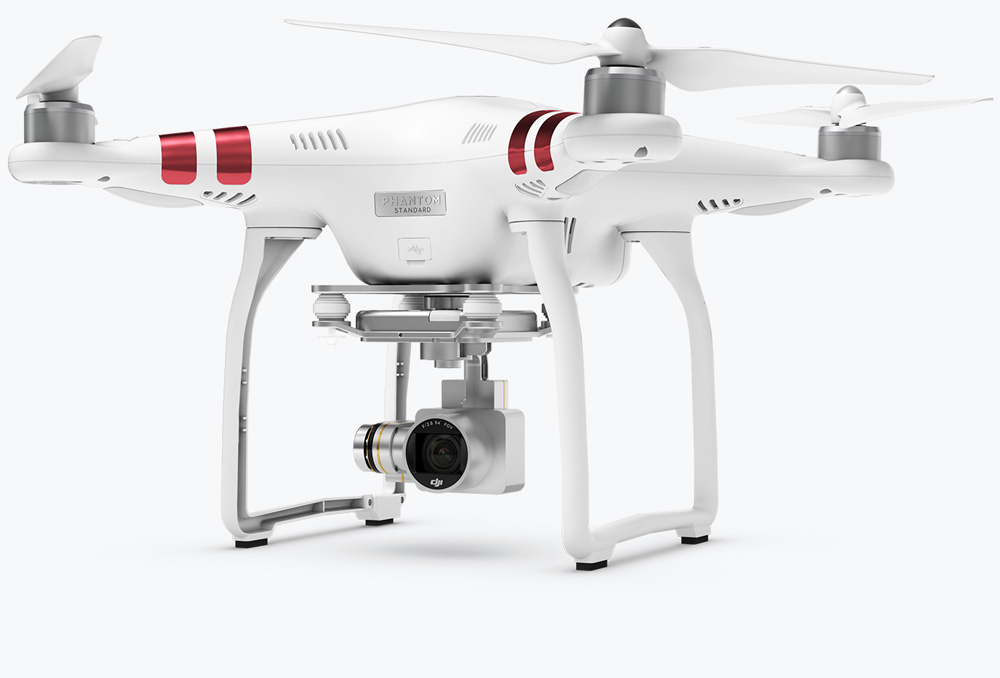
\includegraphics[width=0.7\textwidth]{images/DJI_Phantom_3_Standard.jpg}}
		\caption{DJI Phantom 3 Standard}
	\end{center}
\end{figure}

Die Drone lässt sich auf verschiedenen Wegen steuern. Es gibt die Möglichkeit der klassischen manuellen Steuerung über die Fernbedienung oder man lässt die Drone autonom fliegen. 
\newline
Allgemein ist eine App notwendig, um die Drohne zu steuern und alle Features, welche mit der Drohne kommen, zu nutzen. Hierfür stellt die Firma DJI eine eigene App, die DJI GO App zur Verfügung. Es wird aber auch ein \acf{SDK} bereitgestellt, mit dem sich eigene Apps entwickeln lassen. Durch die durch das \acl{SDK} bereitgestellten Funktionen lassen sich die Features der DJI GO App replizieren und erweitern.
\newline
Das manuelle fliegen lässt sich einfach über die mitgelieferte Fernbedienung realisieren. Die zwei Steuerknüppel dienen hierbei zur Steuerung. Die Funktion der einzelnen Steuerknüppel lässt sich über die DJI eigene App konfigurieren. Hier kann der Nutzer seine Vorlieben einstellen. 
\newline
Um die App bequem während des Fluges bedienen zu können ist an der Fernbedienung eine Halterung montiert in die man das Endgerät, auf der die App ausgeführt wird, befestigen kann. 
\newline
Der Aufbau der Fernbedienung ist in folgender Abbildung zu sehen.
\begin{figure}[H]
	\begin{center}
		{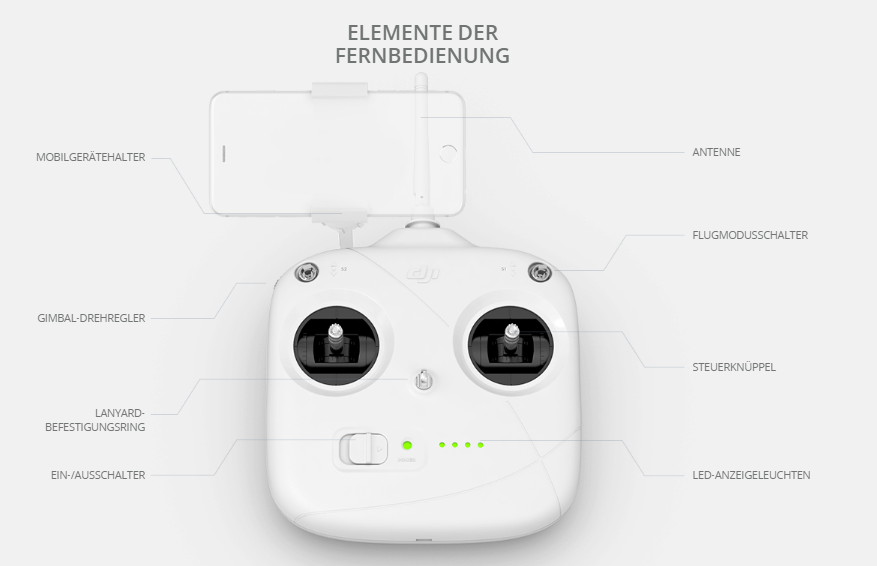
\includegraphics[width=0.5\textwidth]{images/DJI_Fernbedienung.png}}
		\caption{DJI Phantom 3 Standard - Fernbedienung}
	\end{center}
\end{figure}
Die zweite Möglichkeit ist, die Drohne autonom fliegen zu lassen. Hierbei werden sogenannte Waypoints einer Mission hinzugefügt, welche gestartet wird. Die Waypoints beinhalten die Koordinaten mit Längengrad und Breitengrad, sowie der Flughöhe und weiteren Informationen, wie der Fluggeschwindigkeit oder dem Radius mit welchem der Punkt umflogen werden soll. Um den autonomen Flug zu starten wird die Mission gestartet. Während des Fluges erkennt die Drohne über die Kamera Hindernisse und vermeidet eine Kollision mit diesen. 
\newline
Hierbei spielt das \acf{GPS} der Drohne eine wichtige Rolle. Das intelligente System merkt sich den Startpunkt der Drohne. Je nach Einstellung kehrt die Drohne automatisch zum Startpunkt zurück, sollte der Akkustand eine bestimmte Grenze unterschreiten, die Drohne außer Reichweite der Fernbedienung sein oder die return-to-home-Funktion ausgeführt wird.

Die folgende Tabelle gibt eine Übersicht über die wichtigsten, für diese Arbeit relevanten technischen Daten.
\newline
\begin{table}[H]
	\begin{center}
		\begin{tabular}{cc}
			Gewicht & 1216g \\ 
			Diagonale Größe & 350mm \\ 
			max. Steiggeschwindigkeit & 5$\frac{m}{s}$ \\ 
			max. Sinkgeschwindigkeit & 3$\frac{m}{s}$ \\ 
			max. Fluggeschwindigkeit & 16$\frac{m}{s}$ \\
			max. Flughöhe über NN & 6000m \\
			max. Flugzeit & ca. 25 min \\
			Betriebstemperatur & 0° bis 40°C \\
			Positionsbestimmung & GPS \\
			max. Sendereichweite & \begin{tabular}{c}
				FCC: 1000m \\
				CE: 500m \\
				Flughöhe: 120m
			\end{tabular}
		\end{tabular}
	\end{center}
	\caption{DJI Phantom 3 Standard - technische Daten}
\end{table}

\subsection{iPad 3}
Um die in dieser Arbeit zu erstellende App auszuführen und das Produkt zu testen ist ein mobiles Endgerät notwendig. 
\newline
Bei dem mobilen Endgerät handelt es sich um ein iPad der 3. Generation von der Firma Apple.
\newline 
Das iPad hat die Abmessungen:
\begin{itemize}
	\item Höhe: 241,2 mm
	\item Breite: 185,7 mm
	\item Tiefe: 9,4 mm
	\item Gewicht: 652 g
\end{itemize}
Die Bedienfläche ist ein 9,7" großer Multi-Touch Display. Das iPad ist \acl{WLAN} fähig und kann eine Bluetooth Verbindung aufbauen.
\begin{figure}[H]
	\begin{center}
		{\includegraphics[width=0.5\textwidth]{images/iPad3.jpg}}
		\caption{iPad 3}
	\end{center}
\end{figure}


\section{iOS-Appentwicklung}\label{sec:ioS-Appentwicklung}
Bei der Appentwicklung für iOS Geräte bietet sich die Apple eigene Programmiersprache Swift an, welche für die in dieser Arbeit erstellten App auch verwendet wurde. 
\newline
Die Entscheidung für ein für das Projekt sinnvolles Design-Pattern fiel auf das \acf{MVC} Pattern.
\newline
Für die Ansteuerung der DJI-Drone ist das DJI-SDK notwendig, sowie für die Einbindung externer Bibliotheken ist Wissen über Cocoa Pods notwendig.
\newline
Im folgendem werden die genannten Grundlagen in einzelnen Unterkapiteln kurz beschrieben.

\subsection{\acf{MVC}}\label{subsec:MVC}
Das \acs{MVC}-Pattern besteht, wie der Name sagt, aus drei verschiedenen Teilen. Dem Model, dem Controller und der View.
Das Model dient ausschließlich zur Speicherung von Daten. Zum Beispiel werden aktuelle Daten der Anwendung, wie zum Beispiel eine Flugroute in einem Model abgespeichert.
Die View ist für die Darstellung der Inhalte und Daten zuständig. Ebenso ist die View dafür zuständig die Eingaben eines Nutzers an den entsprechenden Controller weiterzuleiten. Die View beinhaltet auch die gesamte \acf{GUI}. 
Der Controller beinhaltet die Anwendungslogik und ist für die Steuerung der Anwendung verantwortlich.
\newline
\begin{figure}[H]
	\begin{center}
		{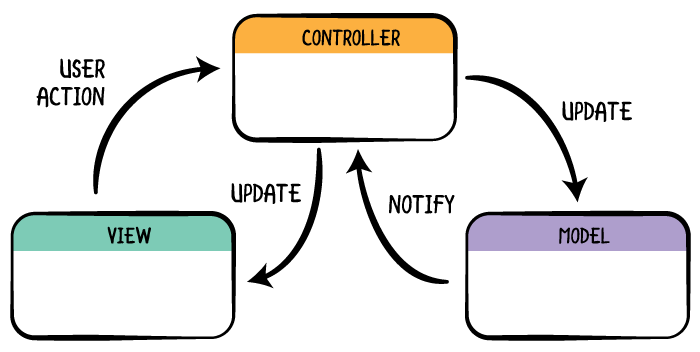
\includegraphics[width=0.5\textwidth]{images/diagram-mvc.png}}
		\caption{MVC Design-Pattern Diagramm \cite{mvc1}}
	\end{center}
\end{figure}
Das \acs{MVC} Pattern kann verschieden streng implementiert werden. In dieser Arbeit wird das Pattern in einer leichten Form angewendet. Es wird sich nicht exakt an die Spezifikation aus der Literatur gehalten.
\newline
\newline
Eine mit Xcode und Swift gschriebenen App hat als Kern eine UIApplication-Klasse. Diese Klasse verarbeitet die Interaktion zwischen System und Objekten der App. Sie verwaltet die geöffneten Views und leitet Ereignisse durch Nutzereingaben oder vom System kommend an die entsprechenden Controller weiter. 
\newline
Die \textit{ViewController} Objekte stellen in einer iOS-Anwendung die Controller des \acs{MVC} Patterns dar. Eine \textit{ViewController}-Klasse verarbeitet Nutzereingaben und aktualisiert die View. 
\newline
Die View ist in der iOS-Programmierung durch sogenannte Storyboards realisiert. 

\subsection{Cocoa}
\subsubsection{\acf{API}}
Cocoa ist eine \acf{API} zur Programmierung unter den \acf{OS} MacOS. Für die Apple \acs{OS} von mobilen Endgeräten, welche über Touch-Displays verfügen, wurde die Cocoa \acs{API} zur CocoaTouch \acs{API} erweitert. CocoaTouch beinhaltet Funktionen für die Nutzereingabe über Eingaben durch Gesten. Somit wird für die Entwicklung von iOS Apps, wie in dieser Arbeit, die CocoaTouch \acs{API} verwendet.
\newline
Die Entwicklung für Apps mit der Cocoa \acs{API} erfolgt mit den Apple eigenen Developer Tools, Xcode, welches im nächsten Kapitel beschrieben wird, und dem Interface Builder. 
\newline
Die hauptsächlich für die \acs{API} gedachten Programmiersprachen sind Objective-C und die Apple eigene Programmiersprache Swift. Die Programmierung in C und C++ ist generell auch möglich. 
\newline
Der Aufbau von Cocoa ist im Allgemeinen einfach gehalten. Cocoa besteht aus drei verschiedenen Frameworks.
\begin{itemize}
	\item \textit{Foundation}: beinhaltet alle relevanten Basisklassen, wie Strings, Arrays, Iterators, et cetera.
	\item \textit{AppKit}: stellt Klassen zur Entwicklung von \acf{GUI} zur Verfügung. Zum Beispiel Buttons, Labels, Menüs, usw..  
	\item \textit{Core Data}: dient zur Erstellung von Objektgraphen.
\end{itemize}
Klassen des Cocoa-Frameworks sind im Quellcode durch die Buchstaben \emph{NS} im Objektnamen zu erkennen. 
\subsubsection{Pods}
CocoaPods ist ein application level dependency manager für Objective-C, Swift und andere Programmiersprachen, welche in XCode laufen. Pods stellt ein Standardformat zum managen von externen Bibliotheken bereit.
\newline
Die Projektabhängigkeiten werden mittels Podfile-Dateien in einem Projekt beschrieben. Im Folgendem ist ein Beispiel zu sehen.
\newline
\begin{lstlisting}[language=ruby, caption={Podfile Beispiel}]
	# platform: iOS, '9.0'
	use_frameworks!
	project 'AirQualityDrone.xcodeproj'
	target 'AirQualityDrone' do
	pod 'DJI-SDK-iOS' '~> 4.4'
	pod 'DJI-UILibrary-iOS', '~> 4.4'
	pod 'CocoaAsyncSocket'
	pod 'DTMHeatmap'
	end
\end{lstlisting}
Um die externen Bibliotheken zu installieren, wird der Befehl \textit{pod install} aufgerufen. Dadurch werden die Quellen der Bibliotheken geladen und das Projekt in Xcode eingerichtet, sodass die Bibliotheken separat gebaut werden. In das Projekt werden die Dateien über eine statische Bibliothek (\textit{libPods.a}).
\begin{figure}[H]
	\begin{center}
		{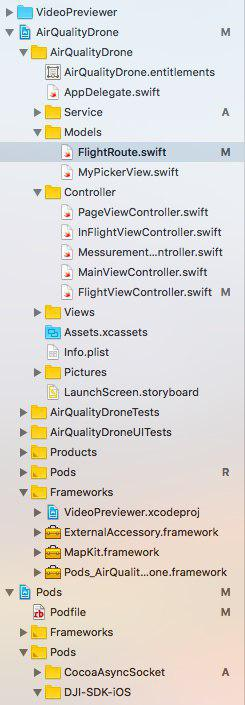
\includegraphics[width=0.5\textwidth]{images/pods.jpg}}
		\caption{Externe Bibliotheken in Xcode}
	\end{center}
\end{figure}

\subsection{Xcode}
Xcode ist eine \acl{IDE} von Apple für das \acs{OS} macOS. Xcode ist für die Entwicklung von Programmen und Apps für macOS, iOS, tvOS und watchOS gedacht. 
Die \acs{IDE} ist BEstandteil der Xcode Tools. 
\newline
Die Xcode Tools beinhalten:
\begin{itemize}
	\item Xcode \acs{IDE}
	\item Interface Builder
	\item Instruments
	\item Xcode Core
	\item Dashcode
	\item Quanz Composer
	\item iPhone Simulator
\end{itemize}
Die iOS App, welche Bestandteil dieser Arbeit ist, wird ausschließlich mit Xcode entwickelt.
Die folgende Abbildung zeigt eine Übersicht der Xcode-Oberfläche.
\begin{figure}[H]
	\begin{center}
		{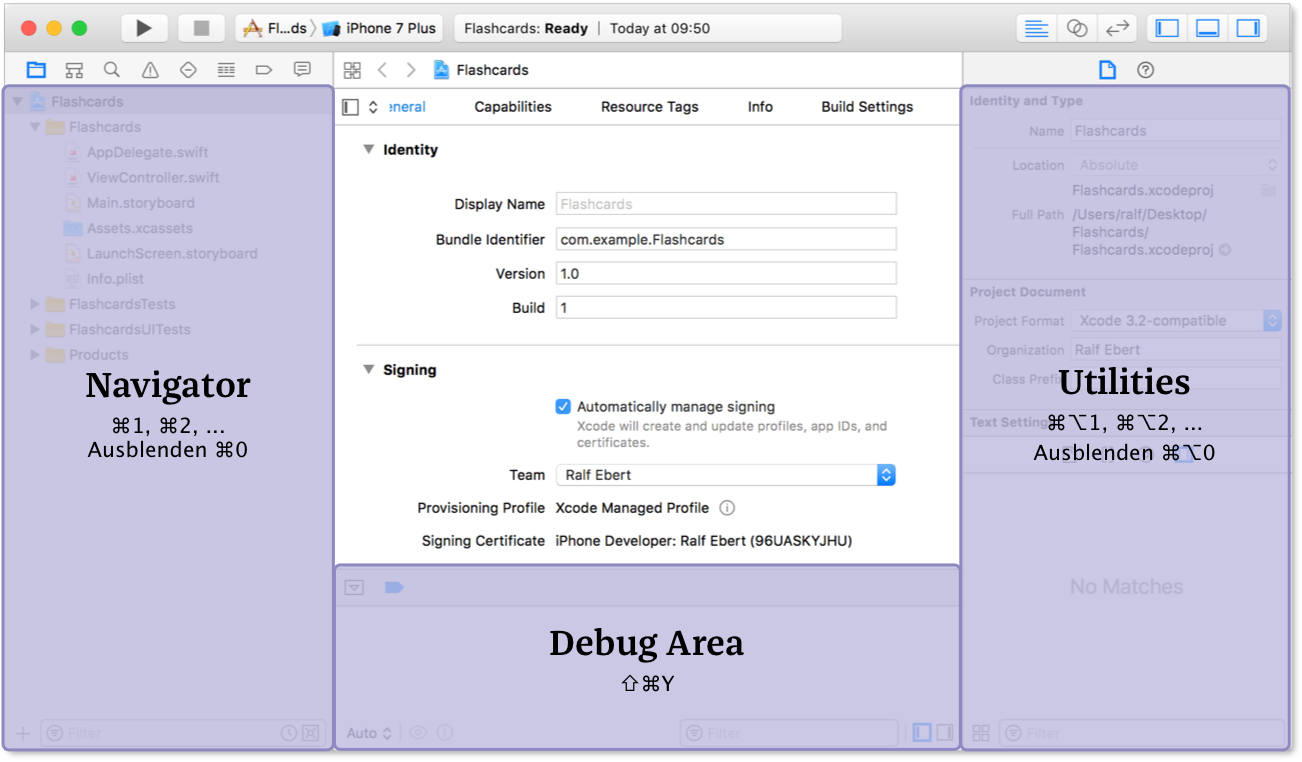
\includegraphics[width=0.8\textwidth]{images/xcode_views.png}}
		\caption{Xcode-Oberfläche}
	\end{center}
\end{figure}
Zentral ist in Xcode der Editor zu finden. Auf der linken Seite befindet sich der Navigator. Unterhalb des Editors befindet sich die Debug Area und auf der rechten Seite die Utilities. Navigator, Debug Area und Utilities lassen sich über die Buttons in der oberen rechten Ecke ausblenden und ermöglichen es so das Editor Fenster größer zu machen.
\newline
Die Projektstruktur ist in Abbildung 2.5 zu sehen. 

\subsection{SWIFT}\label{subsec:SWIFT}
Swift ist eine Programmiersprache des Technik Konzerns Apple. Sie wurde für die Entwicklung von Apps für iOS, Mac, Apple TV und Apple Watch kreiert. Swift ist kostenlos und Open Source. Die Sprache steht unter der Apache 2.0 Open Source Lizenz. Somit kann eine große Community direkt zum Swift Quellcode beitragen. 
\newline
Swift vereint unterschiedliche Konzepte verschiedener Programmiersprachen, wie zum Beispiel Objective-C und Python. Dies führt dazu, dass Sie sich durch Paradigmen wie objektorientiert und imperativ beschreiben lässt. Swift greift Mechanismen, wie Klassen, Vererbung, Closures, Typinferenz, generische Typen, etc., auf, welche von anderen Programmiersprachen bereits bekannt sind. 
\newline
Für die Appentwicklung wurde die Programmiersprache Swift unter der Version 4.1 verwendet. 

\subsection{DJI-\acf{SDK}}\label{subsec:DJI-SDK}
DJI bietet neben dem Verkauf von Drohnen auch noch andere Leistungen an. Hierzu gehören diverse \acs{SDK}, die die Entwicklung von Apps und Programmen für die Drohnen von DJI erleichtern. 
\acs{SDK} die angeboten werden sind:
\begin{itemize}
	\item Mobile SDK
	\item Onboard SDK
	\item Guidance SDK
	\item Payload SDK
\end{itemize}
In dieser Arbeit ist nur das Mobile SDK relevant. 
\newline
Das DJI Mobile SDK unterstützt die Plattformen iOS 9.0 oder höher, sowie Android 5.0.0 oder höher. Da das mobile Endgerät mit einem iOS \acs{OS} läuft, wird in dieser Arbeit die Ausführung des DJI Mobile SDK für iOS verwendet. Hierbei ist die Programmierung in den Sprachen Swift und Objective-C möglich. Wie im Kapitel 2.3.4 erwähnt wird in dieser Arbeit die Programmiersprache Swift 4.1 verwendet. 
\newline
Das SDK bietet verschiedene Kernfunktionalitäten an. Zu diesen wichtigen und nützlichen Features gehört die Obstacle avoidance,  High and low level flight control, Aircraft state through telemetry and sensor data, Live video feed, Pre defined missions, wie Waypoint, HotPoint oder FollowMe und State information und control of Battery und Remote Controller. 
\newline
Für die Entwicklung von \acs{GUI} stellt DJI eine UXLibrary zur Verfügung, welche graphische Elemente für die wichtigsten Funktionen des mobile \acs{SDK} bereitstellt.


		
<<<<<<< HEAD
	% Planung
	%!TEX root = ../dokumentation.tex

%TODO: Einleitungen überarbeiten
\chapter{Projekt-Planung [SB]}\label{cha:Planung}
\section{Anforderungsanalyse}\label{sec:Anforderungsanalyse}
Basierend auf der grundlegenden Idee, eine Drohne mit Sensoren auszustatten, um damit die Luftqualität messen zu können, ist eine Anforderungsanalyse entstanden, welche die Funktionalitäten der ausgestatteten Drohne eindeutig spezifiziert. Die vollständige Anforderungsanalyse findet sich im Anhang.
\subsection{Muss-Kriterien}\label{subsec:MussKrit}
Im Folgenden werden zunächst die Kernanforderungen näher erläutert und warum diese absolute Priorität genießen.
\newline
\begin{enumerate}[label=\roman*.]
	\item Der Drohnenflug muss mittels der App gestartet werden können
	\item Die Flugroute muss mittels der App festgelegt werden können
	\item Der Drohnenflug muss mittels der App abgebrochen werden können
	\item Die Messwerte müssen über die App einsehbar sein
	\item Die Messwerte müssen über die App exportierbar sein
	\item Die App muss dem Benutzer ermöglichen, einen Flugbereich auf einer Karte zu markieren
	\item Die App muss dem Benutzer ermöglichen, die Flughöhe für die Messung auszuwählen
	\item Die auf der Karte ausgewählte Flugroute muss gestartet werden können
	\item Die App muss dem Benutzer ermöglichen, aus verschiedenen Messhäufigkeiten auszuwählen
	\item Die Drohne muss Feinstaub messen können (2.5 \& 10 $\mu m$)
	\item Die Drohne muss Druck messen können
	\item Die Drohne muss Feuchtigkeit messen können
	\item Die Drohne muss Temperatur messen können
	\item Die Drohne muss Stickoxide (NO\textsubscript{x}) messen können	
\end{enumerate}
Wie aus den obigen Anforderungen ersichtlich ist, liegt das Hauptaugenmerk darauf, die Drohne mittels einer App ansprechen und steuern zu können, während die Sensoren die gemessenen Umgebungsdaten an die App senden, damit diese dort angezeigt werden. Das Senden sowie das Verarbeiten der Sensordaten geschieht mittels des Bosch \acf{XDK}, welches als Schnittstelle zwischen den Sensoren und der App dient.
\subsection{Soll-Kriterien}\label{subsec:SollKrit}
In Ergänzung zu diesen kritischen Anforderungen, werden nachfolgend weitere Funktionalitäten beschrieben, welche ebenfalls für sinnvoll erachtet wurden, die jedoch nicht besonders kritisch sind. Die ergänzten Funktionalitäten umschließen weitere zu messende Größen sowie einige graphischen Verbesserungen, die eine übersichtlichere Rückmeldung zur laufenden Messung bieten sollen.
\newline
\begin{enumerate}[label=\roman*.]
	\item Die Messwerte sollen in der App visualisiert werden 	
	\item Die App soll die Messdaten in Abhängigkeit der Höhe zweidimensional auf der Karte anzeigen können
	\item Basierend auf dem auswählbaren Flugbereichs auf einer Karte, soll die App eine Flugroute automatisch berechnen können.
	\item Die App soll dem Benutzer ermöglichen, Bereiche explizit aus dem Flugbereich auszuschließen
	\item Die App soll die Drohnenposition während des Fluges auf einer Karte anzeigen
	\item Die App soll eine Fortschrittsanzeige zur laufenden Messung bieten
	\item Die App soll einen permanenten Video-Stream während des Drohnenflugs anzeigen
	\item Die Drohne soll Kohlenstoffdioxid (CO\textsubscript{2}) messen können
	\item Die Drohne soll Ozon (O\textsubscript{3}) messen können	
\end{enumerate}
\subsection{Kann-Kriterien}\label{subsec:KannKrit}
Sollten die oben genannten Funktionalitäten noch immer nicht den Rahmen des Projektes sprengen, sind mit den folgenden Anforderungen noch einige optionale Funktionalitäten erfasst, die potentiell einen weiteren Mehrwert liefern.
\newline
\begin{enumerate}[label=\roman*.]
	\item Der Benutzer kann in der App Flugrouten erstellen, speichern und abrufen 
	\item Der Benutzer kann in der App Messprofile erstellen, speichern und abrufen 
	\item Die App kann die Benutzerprofile exportieren können
	\item Die App kann durch Verrechnung von verbleibendem Akkustand und der vorgegebenen Flugroute einen Warnhinweis an den Benutzer geben, dass die Messung potenziell nicht ausgeführt werden kann
	\item Die App kann die Messdaten dreidimensional darstellen
	\item Die Drohne kann Kohlenstoffmonoxid (CO) messen können
	\item Die Drohne kann Schwefeldioxid (SO\textsubscript{2}) messen können
	\item Die Drohne kann flüchtige organische Verbindungen (VOC) messen können
	\item Die Drohne kann Methan (CH\textsubscript{4}) messen können	
	\item Der Anwender kann die Messdaten mittels der App einem Server übermitteln können	
\end{enumerate}
\section{Aufgabenteilung}\label{sec:Aufgabenteilung}
Um eine klare Trennung und Zuordnung der Aufgaben zu erreichen, ist das Projekt grob in 2 Bereiche eingeteilt. 
\newline
Die erste Komponente ist die iOS-App, welche für die Ansteuerung der Drohne, sowie die Visualisierung der Messdaten zuständig ist.
\newline
Die zweite Komponente ist der Entwurf des Messsystems mit allen Sensoren, deren Verschaltung und die Verarbeitung deren Daten mittels des Bosch \acs{XDK}.
\newline
\newline
Alle Aufgaben hinsichtlich der App werden von Julian Riegger bearbeitet, während alle Aufgaben zum Messsystem von Sebastian Breit bearbeitet werden.
\section{Zeitplan}\label{sec:Zeitplan}
In Ergänzung zu der bereits erwähnten Aufgabenteilung, wird zur besseren Planung und Nachverfolgung des Projektes ein Zeitplan verwendet, der auf einer hohen Abstraktionsebene die Aufgaben zeitlich einplant. Der Zeitplan ist mittels des frei verfügbaren Online-Tools Agantty erstellt, mit dessen Hilfe man einfach und unkompliziert Projekt-Pläne erstellen kann und dabei spezifische Aufgaben bestimmten Personen zuordnen kann. 
\newline 
\newline
Abbildung ~\ref{fig:Zeitplan} zeigt den erstellten Zeitplan.
\begin{figure}[H]
	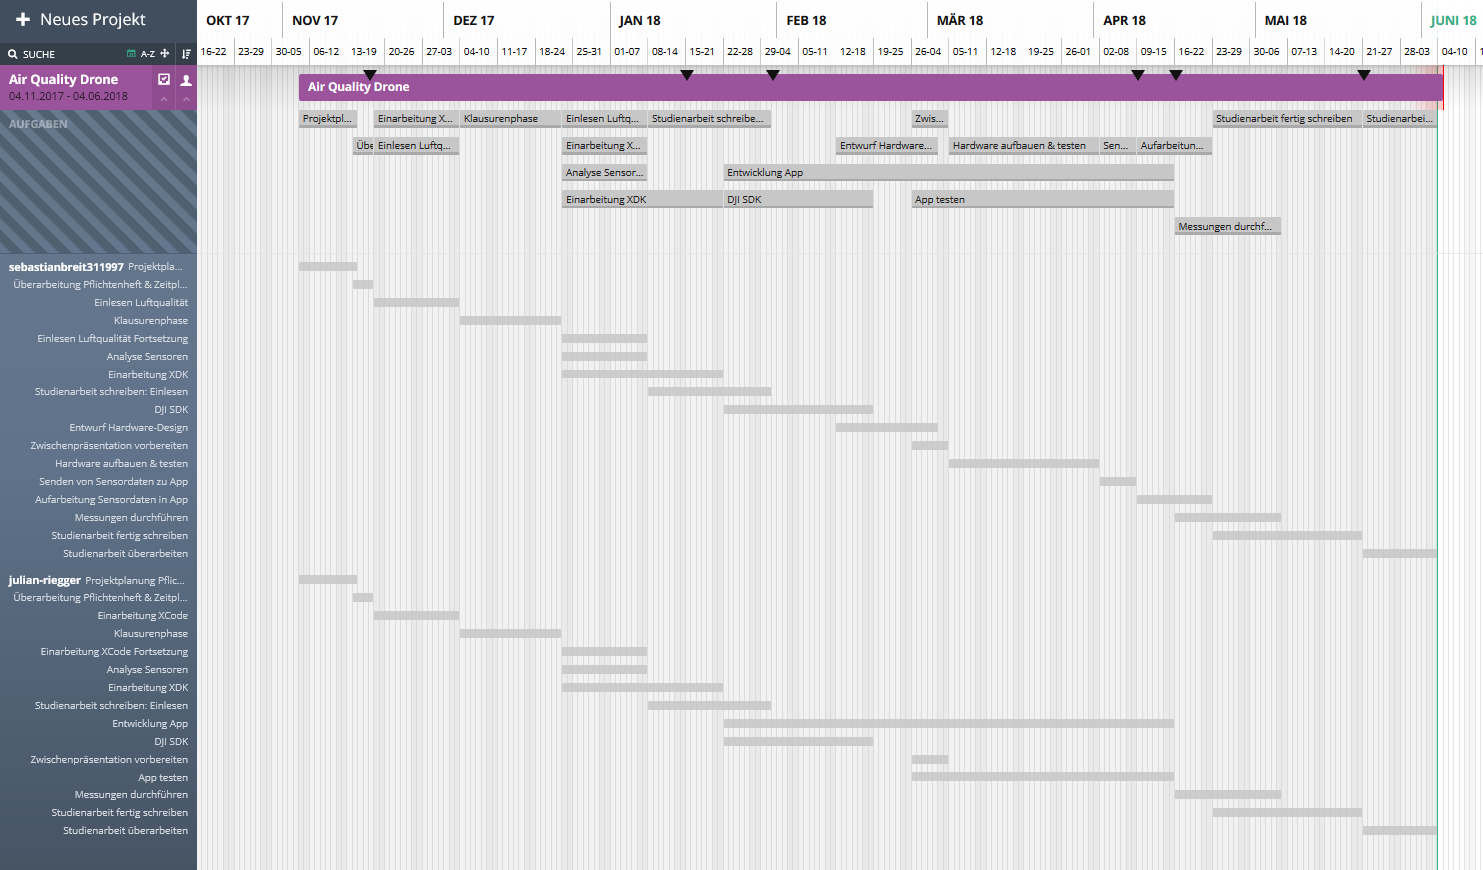
\includegraphics[width=\textwidth]{images/Zeitplan.png}	
	\caption{Zeitplan}
	\label{fig:Zeitplan}
\end{figure}



	
	% Setup
	%!TEX root = ../dokumentation.tex

%TODO: Einleitung überarbeiten
\chapter{Setup}\label{cha:Setup}
Lorem ipsum \ac{OS} Ubuntu  dolor sit amet, consetetur sadipscing elitr, sed diam nonumy eirmod tempor invidunt ut labore et dolore magna aliquyam erat, sed diam voluptua. At vero eos et accusam et justo duo dolores et ea rebum. Stet clita kasd gubergren, no sea takimata sanctus est Lorem ipsum dolor sit amet. Lorem ipsum dolor sit amet, consetetur sadipscing elitr, sed diam nonumy eirmod tempor invidunt ut labore et dolore magna aliquyam erat, sed diam voluptua. At vero eos et accusam et justo duo dolores et ea rebum. Stet clita kasd gubergren, no sea takimata sanctus est Lorem ipsum dolor sit amet. Lorem ipsum dolor sit amet, consetetur sadipscing elitr, sed diam nonumy eirmod tempor invidunt ut labore et dolore magna aliquyam erat, sed diam voluptua. At vero eos et accusam et justo duo dolores et ea rebum. Stet clita kasd gubergren, no sea takimata sanctus est Lorem ipsum dolor sit amet. 

Duis autem vel eum iriure dolor in hendrerit in vulputate velit esse molestie consequat, vel illum dolore eu feugiat nulla facilisis at vero eros et accumsan et iusto odio dignissim qui blandit praesent luptatum zzril delenit augue duis dolore te feugait nulla facilisi. Lorem ipsum dolor sit amet, consectetuer adipiscing elit, sed diam nonummy nibh euismod tincidunt ut laoreet dolore magna aliquam erat volutpat. 

Ut wisi enim ad minim veniam, quis nostrud exerci tation ullamcorper suscipit lobortis nisl ut aliquip ex ea commodo consequat. Duis autem vel eum iriure dolor in hendrerit in vulputate velit esse molestie consequat, vel illum dolore eu feugiat nulla facilisis at vero eros et accumsan et iusto odio dignissim qui blandit praesent luptatum zzril delenit augue duis dolore te feugait nulla facilisi. 

\newpage
\begin{lstlisting}[language=bash, caption={Konfiguration des Hadoop Users}, label=lis:KonfHadoopUser]
# Create usergroup and user
sudo addgroup hadoop
sudo adduser -ingroup hadoop hduser

# login as hadoop user and create rsa key
su - hduser
ssh-keygen -t rsa -P ""

# add to authorized keys
cat $HOME/.ssh/id_rsa.pub >> $HOME/.ssh/authorized_keys

# Initial login on host via ssh
ssh localhost
\end{lstlisting}

\begin{lstlisting}[language=bash, caption={Herunterladen und entpacke von Hadoop}, label=lis:HerunterladenUndEntpacken]
$ cd /usr/local
$ sudo wget http://apache.openmirror.de/hadoop/common/current
            /hadoop-2.7.1.tar.gz
$ sudo tar xfz hadoop-2.7.1.tar.gz
$ sudo mv hadoop-2.7.1 hadoop
$ sudo chown -R hduser:hadoop hadoop
\end{lstlisting}

\newpage
\begin{lstlisting}[language=bash, caption={Umgebungsvariablen für Hadoop}, label=lis:Umgebungsvariablen]
# Java
export JAVA_HOME=/usr/lib/jvm/java-7-openjdk-amd64

# Hadoop
export HADOOP_INSTALL=/usr/local/hadoop
export PATH=$PATH:$HADOOP_INSTALL/bin
export PATH=$PATH:$HADOOP_INSTALL/sbin
export HADOOP_MAPRED_HOME=HADOOP_INSTALL
export HADOOP_COMMON_HOME=HADOOP_INSTALL
export HADOOP_HDFS_HOME=HADOOP_INSTALL
export HADOOP_YARN_HOME=HADOOP_INSTALL
\end{lstlisting}

\begin{figure}[h]
	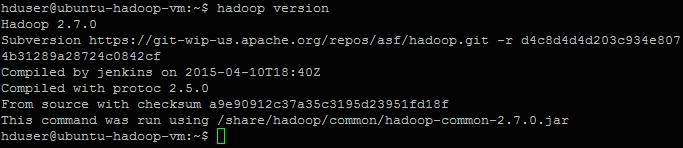
\includegraphics[width=1\textwidth]{hadoop_version.png}
	\caption{Ergebnis für die Kommandozeileneingabe \textit{hadoop version}}
	\label{fig:ErgebnisKomandozeileneingabe}
\end{figure}

\pagebreak
\begin{lstlisting}[language=XML, caption=Konfiguration in der core-site.xml, label=lis:KonfCoreSite]
<configuration>
	<property>
		<name>fs.defaultFS</name>
		<value>hdfs://localhost:9000</value>
	</property>
</configuration>
\end{lstlisting}
	
	% Architektur	
	%!TEX root = ../dokumentation.tex

\chapter{Architektur [SB]}\label{cha:Architektur}
\section{Architektur Konzept}\label{sec:Architektur Konzept}
Wie in Abbildung ~\ref{fig:Architektur_grob} zu sehen ist, besteht das System im Kern aus 3 Komponenten. Die Drohne, das \acs{XDK} sowie das Tablet sind alle mit dem \acs{WLAN} der Drohne verbunden. Über dieses läuft dann die komplette Kommunikation zwischen den einzelnen Komponenten ab. Die App kommuniziert über das \acs{DJI}-\acs{SDK} mit der Drohne, das \acs{XDK} baut eine UDP-Verbindung zur App auf, über die es die gemessenen Sensordaten schicken kann.
\begin{figure}[H]
	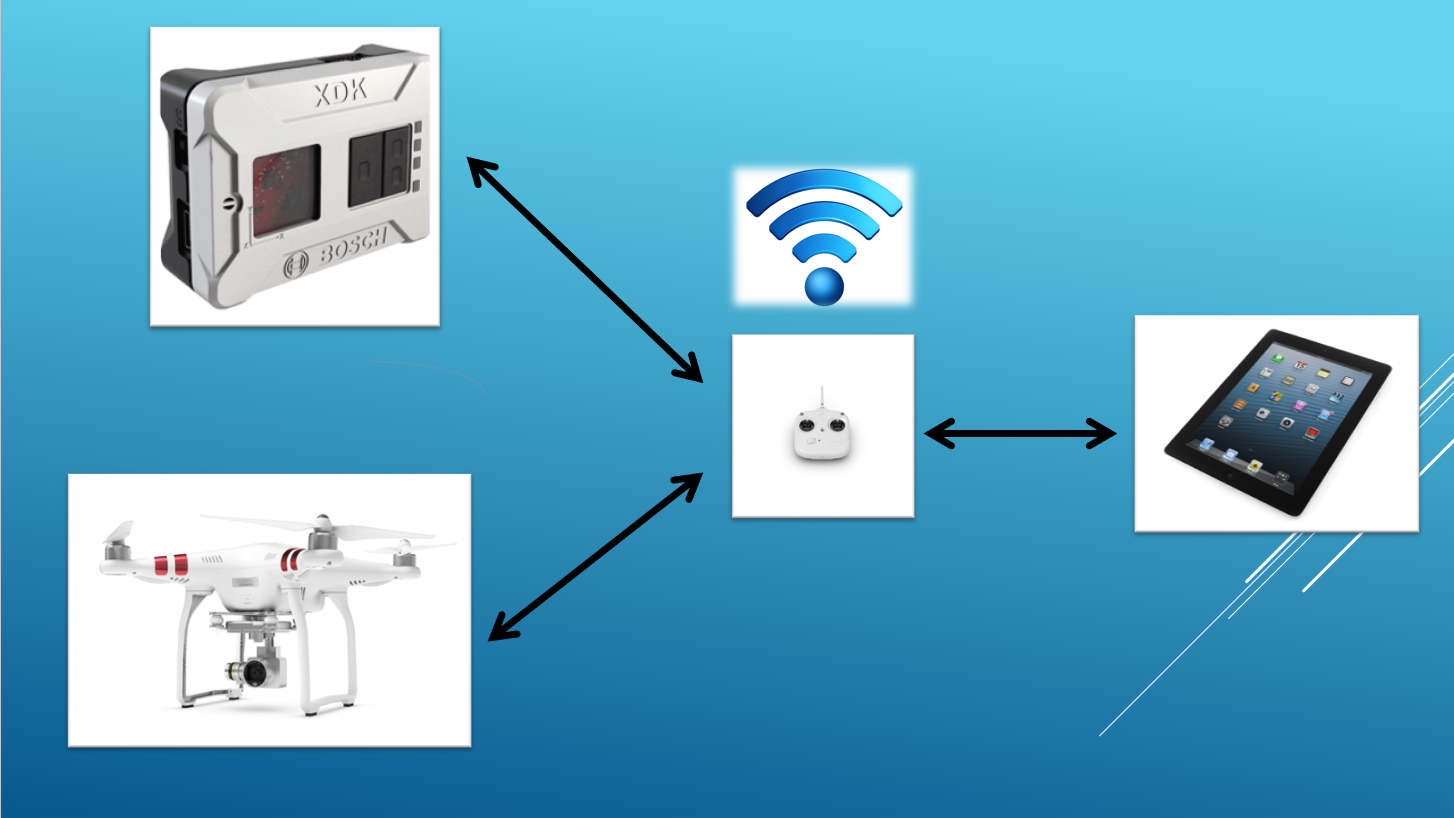
\includegraphics[width=\textwidth]{images/Architektur_grob.png}	
	\caption{Architektur allgemein}
	\label{fig:Architektur_grob}
\end{figure}

\section{Lesen der Sensordaten}\label{sec:Lesen der Sensordaten}
Abbildung ~\ref{fig:Architektur_fein} zeigt schematisch das Auslesen der Sensordaten am \acs{XDK}. Das \acs{XDK} ist mit dem dazu passenden Extension Board direkt über eine serielle Schnittstelle verbunden, über die es die Messwerte der externen Sensoren empfängt. 
\newline
Für die analogen Sensoren werden prinzipiell deren Spannungspegel am Ausgang auf einen Multiplexer geleitet, der in Abhängigkeit des Signales vom Extension Board entscheidet, welcher Sensor-Ausgang auf den Ausgang des Multiplexers übertragen wird. Die Ansteuerung des Multiplexers erfolgt auf Seiten der Software auf dem \acs{XDK}. Darin wird festgelegt, wie genau die \acs{GPIO}-Pins des Extension-Boards zu beschalten sind. Abschließend wird dann der Wert am Ausgang des Multiplexers vom Analog-Digital-Wandler des Extension Boards erfasst und an das \acs{XDK} übermittelt.
\newline
Die Messwerte des Feinstaub-Sensors SDS011 können lediglich über \acs{UART} erfasst werden. Aus diesem Grund wird der Sensor nicht mit dem Multiplexer verbunden, sondern direkt, beziehungsweise nach Anpassung des Spannungs-Pegels, mit dem Extension Board verbunden. In der Software des \acs{XDK} lässt sich dann konfigurieren, dass die mit dem Sensor verbundenen Pins für \acs{UART} genutzt werden sollen, womit die Messwerte direkt in digitaler Form am XDK erfasst werden können.
\newline
Aufgrund dessen, dass der Feinstaub-Sensor die gemessenen Daten höchstens im Sekundentakt per UART übermitteln kann, ist die maximale Messdichte ebenfalls auf 1 Messung pro Sekunde beschränkt. Damit die 5 analogen Sensoren auch mindestens einmal in diesem Intervall ihre Daten an das XDK weitergeben, werden die \acs{GPIO}-Pins von der Software alle 100ms geändert, sodass immer ein anderer Sensor am Analog-Digital-Wandler anliegt. 
\newline
Sind nun in einer Sekunde alle Daten einmal gemessen, so sendet das \acs{XDK} diese sofort per \acs{UDP} über das \acs{WLAN} der Drohne an die iOS-Applikation, wo die Messdaten dann visualisiert werden können.

\begin{figure}[H]	
	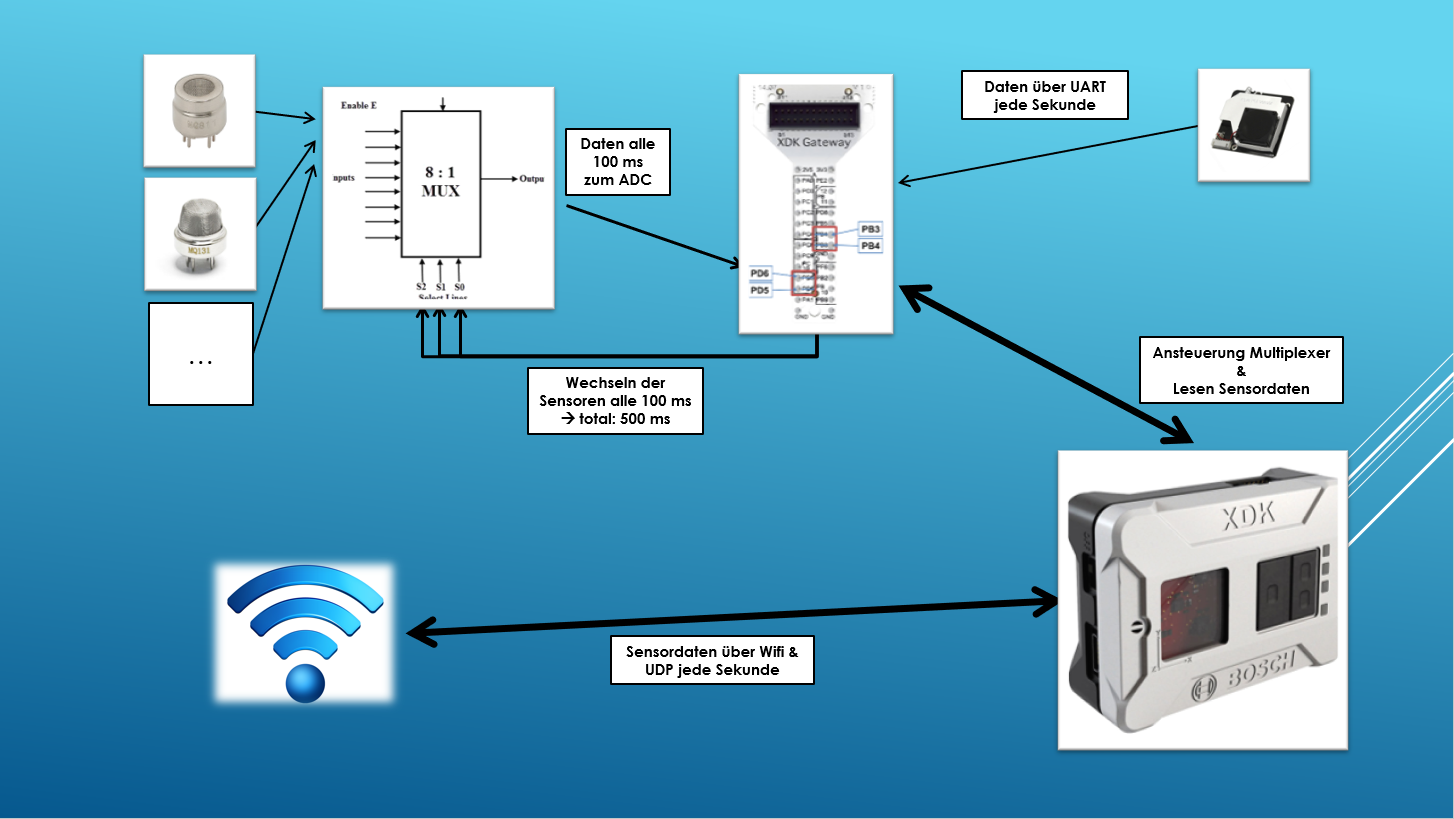
\includegraphics[width=\textwidth]{images/Architektur_fein.png}	
	\caption{Architektur Sensorik}
	\label{fig:Architektur_fein}
\end{figure}

Wie wir basierend auf der vorangegangenen Tabelle erkennen können, liefert kein Sensor einen Pegel von 2,5V, wie er vom \acs{XDK} benötigt wird. Damit die von den Sensoren gelieferten Daten nun also verarbeitet werden können, müssen die Pegel angepasst werden. Um dies zu erreichen, wird ein Operationsverstärker verwendet, der die Ausgangsspannung um die Hälfte reduziert. Näheres zu diesem Prozess in Abschnitt ~\ref{subsec:Operationsverstärker}.
Neben der Anpassung der Pegel ist noch ein weiterer Schritt erforderlich, um die analogen Sensordaten lesen zu können. Bedingt dadurch, dass 5 analoge Sensoren auszuwerten sind und dafür lediglich 2 Pins verfügbar sind, welche als \acs{ADC} genutzt werden können, müssen mehrere der Sensoren mit einem \acs{ADC} gemessen werden. Um dies zu ermöglichen, werden die Sensordaten mit Hilfe eines Multiplexers in verschiedenen Zeitschlitzen übermittelt. Um den Multiplexer anzusteuern werden dabei die \acs{GPIO}-Pins des \acs{XDK} verwendet. Die genaue Beschreibung hierzu lässt sich in Abschnitt ~\ref{subsec:Multiplexer} finden.

Neben den 5 analogen Sensoren muss auch das Signal des Feinstaub-Sensors angepasst werden, welcher die Daten seriell über \acs{UART} mit 3,3V übermittelt. Um dieses Signal auf die erforderlichen 2,5V umzuwandeln, wird ein Pegelwandler verwendet, der diskrete Pegel konvertieren kann. Dies wird in Abschnitt ~\ref{subsec:Pegelwandler} näher beschrieben.

\section{Schaltungsdesign}\label{sec:Schaltungsdesign}
Da die Sensoren aus Tabelle ~\ref{tab:Sensoren} Ausgangs-Spannungen zwischen 0V und 5V liefern, müssen diese Spannungen noch umgewandelt werden, bevor sie mit dem Extension Board und somit dem XDK verbunden werden dürfen. Aus diesem Grund werden mehrere Pegel-Wandler und Operationsverstärker eingesetzt, damit die einzelnen Komponenten kompatibel werden.
\newline
In diesem Abschnitt wird nun näher auf das konkrete Schaltungs-Design eingegangen, wie die Bauteile elektrisch miteinander verbunden sind und wie die Spannungen umgewandelt werden, sodass die einzelnen Komponenten miteinander kommunizieren können. Ein Überblick über das gesamte Schaltungslayout lässt sich im Anhang in Abschnit ~\ref{sec:Schaltungs-Layout_komplett} finden.
\newline
Die gezeigten Schaltungs-Layouts und die dabei verwendeten Komponenten sind mit Hilfe der gratis \acf{CAD}-Software PCBWeb entworfen worden, die sowohl zum Entwurf schematischer Schaltpläne, als auch zur Erstellung von \acf{PCB}-Layouts verwendet werden kann.
\subsection{Extension-Board}\label{subsec:Extension-Board}
\begin{figure}[H]
	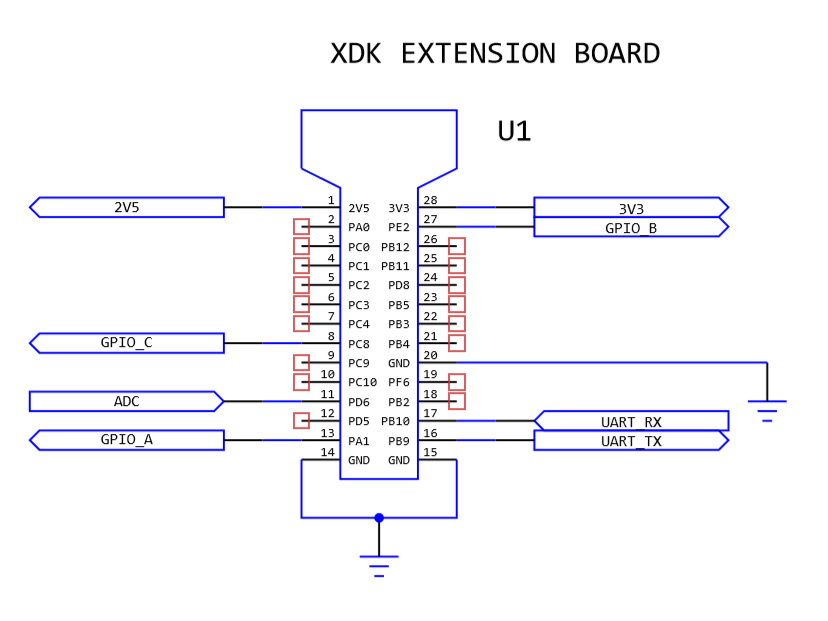
\includegraphics[width=\textwidth]{images/Layout_XDK.png}	
	\caption{Layout Extension-Board}
	\label{fig:Layout_ExtensionBoard}
\end{figure}
Abbildung ~\ref{fig:Layout_ExtensionBoard} zeigt ganz konkret die Beschaltung des Boards und wie die angeschlossenen Pins verwendet werden. Die Pins 1 und 28 dienen als Spannungsquelle für alle Komponenten, die Spannungen von 2,5V oder 3,3V benötigen. 
\newline
Die Pins PA1, PE2 sowie PC8 werden als \acs{GPIO}-Pins benutzt, mit denen der Multiplexer angesteuert wird.
\newline
PD6 ist konfiguriert, um als Analog-Digital-Wandler die Spannungen der analogen Sensoren zu digitalisieren. Dazu wird er nach einer Anpassung des Spannungspegels mit dem Multiplexer verbunden.
\newline
Die beiden Pins PB9 und PB10 sind für \acs{UART} konfiguriert und werden mit letztlich mit dem Feinstaub-Sensor SDS011 verbunden.
\subsection{Multiplexer}\label{subsec:Multiplexer}
\begin{figure}[H]
	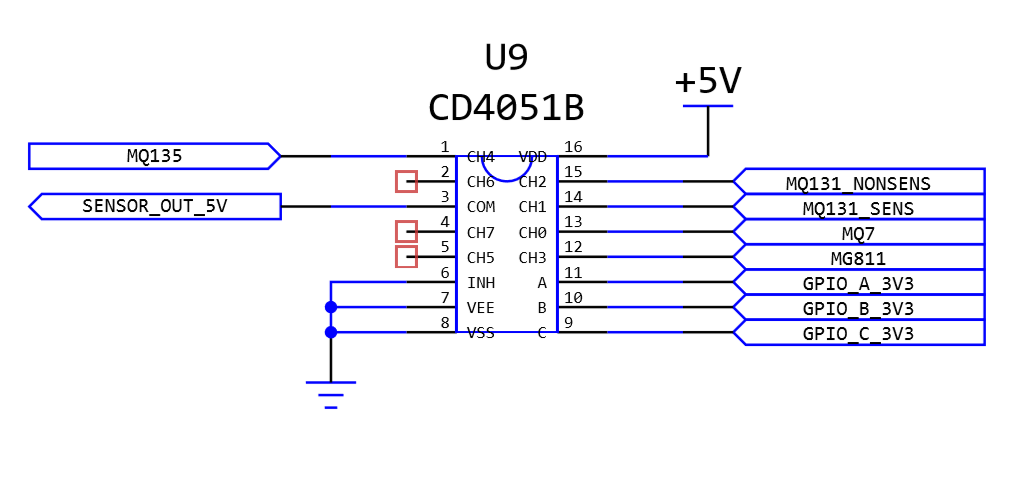
\includegraphics[width=\textwidth]{images/Layout_Multiplexer.png}	
	\caption{Layout Multiplexer}
	\label{fig:Layout_Multiplexer}
\end{figure}
Damit der Multiplexer die Spannungs-Werte der Sensoren auf den Ausgang durchschalten kann, benötigt er an den Steuerungs-Eingängen A, B und C Spannungen von mindestens 3,3V. Aus diesem Grund können nicht einfach die \acs{GPIO}-Pins des Extension-Boards direkt mit dem Multiplexer verbunden werden, da diese lediglich 2,5V liefern. Damit diese Pegel angepasst werden, werden die \acs{GPIO}-Pins zunächst mit einem Pegelwandler verbunden, wie in Abbildung ~\ref{fig:Layout_LevelShifter} zu sehen ist.
\newline
Wenn somit die Steuerung des Multiplexers funktioniert, wird abhängig von der Beschaltung der Pins A, B und C der Ausgang COM auf den passenden Eingangskanal durchgeschaltet. Tabelle ~\ref{tab:MultiplexerLogic} zeigt die logischen Verknüpfungen.
\begin{table}[H]
	\begin{center}
			\begin{tabular}{|c|c|c|c|}
				\hline
				A & B & C & Output (Channel)  \\ \hline \hline
				
				0 & 0 & 0 & 0 \\ \hline 
				0 & 0 & 1 & 1 \\ \hline 
				0 & 1 & 0 & 2 \\ \hline 
				0 & 1 & 1 & 3 \\ \hline 
				1 & 0 & 0 & 4 \\ \hline 
				1 & 0 & 1 & 5 \\ \hline 
				1 & 1 & 0 & 6 \\ \hline 
				1 & 1 & 1 & 7 \\ \hline 							
			\end{tabular}
	\end{center}
	\caption{Logische Ansteuerung Multiplexer ~\cite{DataSheet.CD4051B}}
	\label{tab:MultiplexerLogic}
\end{table}
Ist nun ein bestimmter Eingangskanal auf den Ausgang durchgeschaltet, so kann das Signal trotzdem noch nicht mit dem \acs{ADC} verbunden werden, da die Spannungswerte des Signals zwischen 0V und 5V liegen können. Da das XDK nur Spannungen bis zu 2,5V verträgt, muss die Spannung auf diesen Bereich umgewandelt werden. Wie dies zu erreichen ist, wird in Abschnitt ~\ref{subsec:Operationsverstärker} näher erläutert.
\subsection{Pegelwandler}\label{subsec:Pegelwandler}
\begin{figure}[H]
	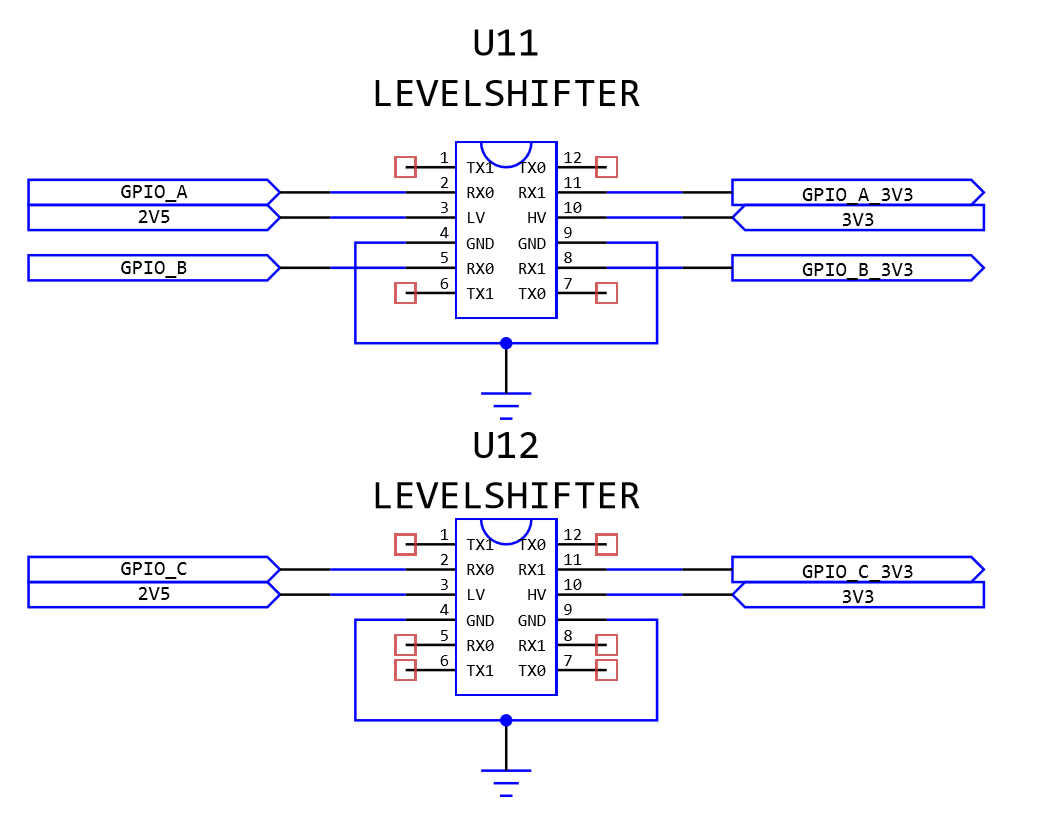
\includegraphics[width=\textwidth]{images/Layout_LevelShifter.png}	
	\caption{Layout Pegelwandler}
	\label{fig:Layout_LevelShifter}
\end{figure}
Wie bereits zuvor erwähnt werden die beiden Pegelwandler benutzt, um die Spannung der von den \acs{GPIO}-Pins eingehenden Signale auf 3,3V anzuheben, damit der Multiplexer diese verarbeiten kann.
\subsection{Operationsverstärker}\label{subsec:Operationsverstärker}
Wie im Abschnitt ~\ref{subsec:Multiplexer} erwähnt, muss das Ausgangssignal des Multiplexers aus dem Intervall von 0V bis 5V in das Intervall von 0V bis 2,5V konvertiert werden. Dies geschieht mittels eines Operationsverstärkers und der dazugehörigen Grundschaltung des invertierenden Verstärkers, welche in Abbildung ~\ref{fig:InvertierenderVerstärker} zu sehen ist. ~\cite{DataSheet.LM158N}
\begin{figure}[H]
	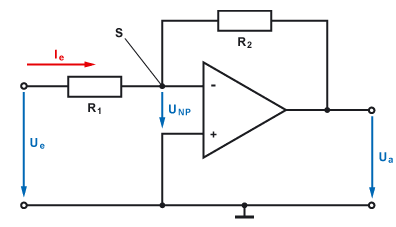
\includegraphics{images/InvertierenderVerstaerker.png}	
	\caption{Invertierender Verstärker}
	\label{fig:InvertierenderVerstaerker}
\end{figure}
Laut der Grundgleichung des invertierenden Verstärkers wird der Verstärkungsfaktor V berechnet mit:
\[ V_u = \frac{U_a}{U_e} = -\frac{R_2}{R_1} \]
Um nun eine Dämpfung um den Faktor 2 zu erhalten, beschalten wir einen ersten Operationsverstärker mit \(R_1 = 20K\Omega\) und \(R_2 = 10K\Omega\). Da dadurch das Signal allerdings im Intervall von -2,5V bis 0V liegt, wird ein weiterer Operationsverstärker damit beschaltet, der die Wiederstände \(R_3 = 10K\Omega\) und \(R_4 = 10K\Omega\) besitzt, wodurch das Signal erneut invertiert wird und es somit im korrekten Intervall erscheint. 
\newline
Diese schematische Beschaltung ist in Abbildung ~\ref{fig:Layout_OP} zu erkennen.
\begin{figure}[H]
	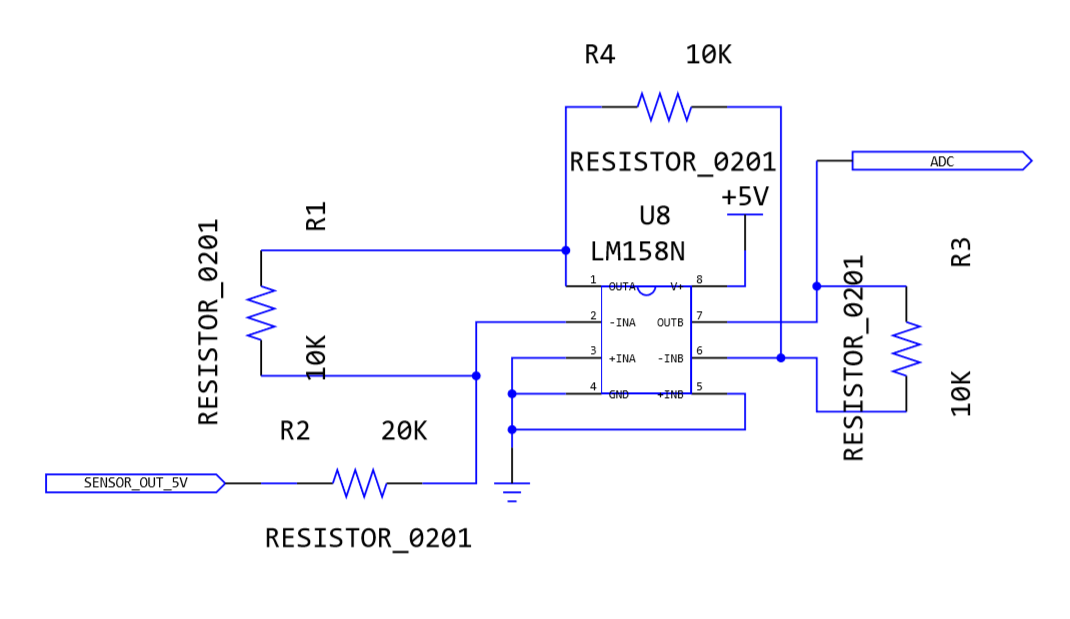
\includegraphics[width=\textwidth]{images/Layout_OP.png}	
	\caption{Layout Operationsverstärker}
	\label{fig:Layout_OP}
\end{figure}
\subsection{Feinstaub-Sensor}\label{subsec:Feinstaub-Sensor}
Abbildung ~\ref{fig:Layout_SDS011} zeigt die Beschaltung des Feinstaub-Sensors. Man kann erkennen, dass auch hier die Signale des Sensors zunächst auf einen Pegelwandler geschickt werden, damit dieser die Spannungspegel von 3,3V auf 2,5V umwandelt. Nach der Umwandlung werden die daraus resultierenden Signale direkt mit den entsprechenden Pins am \acs{XDK} Extension Board verbunden, an denen die digitalisierten Messwerte über \acs{UART} ausgelesen werden.
\begin{figure}[H]
	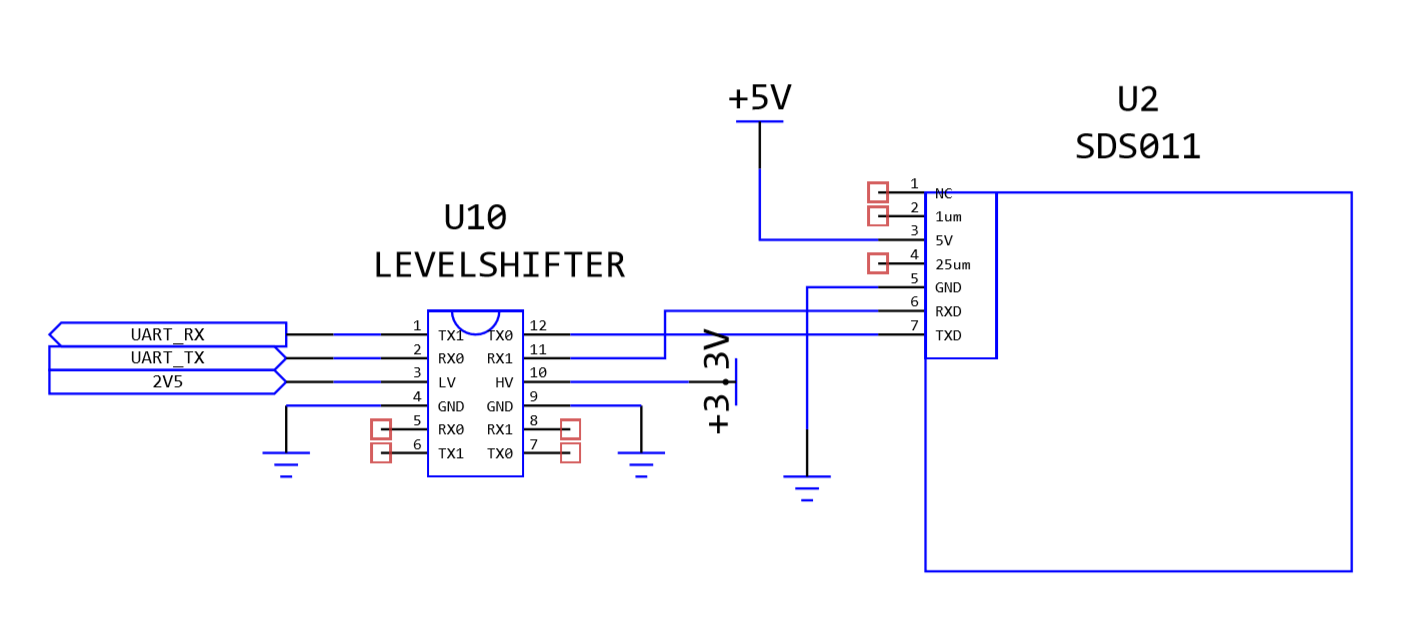
\includegraphics[width=\textwidth]{images/Layout_SDS011.png}	
	\caption{Layout Feinstaub-Sensor}
	\label{fig:Layout_SDS011}
\end{figure}
\subsection{Layout analoger Sensor}\label{subsec:Layout analoger Sensor}
Zum Abschluss der Schaltungs-Layouts zeigt Abbildung ~\ref{fig:Layout_Sensor_Example} eine beispielhafte Beschaltung eines der analogen Sensoren. Da diese bei allen anderen Sensoren praktisch gleich aussieht, wird hier nur die Abbildung des MQ7-Sensors zur Veranschaulichung dargestellt. Die vollständigen Layouts der Sensoren finden sich im kompletten Schaltungs-Layout im Anhang in Abschnitt ~\ref{sec:Schaltungs-Layout_komplett}.
\begin{figure}[H]
	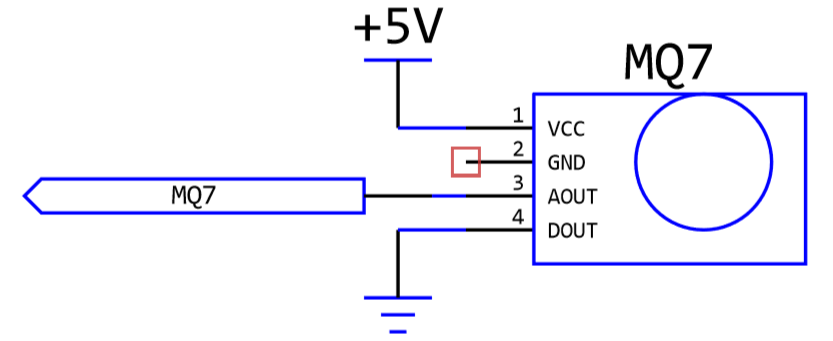
\includegraphics[width=8cm]{images/Layout_Sensor_Example.png}	
	\caption{Layout analoger Sensor}
	\label{fig:Layout_Sensor_Example}
\end{figure}	
	
	% Umsetzung
	%!TEX root = ../dokumentation.tex

\chapter{XDK Code}\label{cha:XDK Code}
Zur Steuerung und zum Erfassen der Messwerte der Sensoren wird C Code verwendet, der compiliert auf das Bosch \acs{XDK} aufgespielt wird. Wie in Kapitel ~\ref{sec:Bosch XDK} erwähnt, läuft auf dem \acs{XDK} das Echtzeitbetriebssystem FreeRTOS, das Programme in verschiedene Tasks unterteilt. Auch der Code zum Verwalten der Sensoren ist in diverse Tasks unterteilt, welche alle quasi-parallel ablaufen.
\newline
In den folgenden Abschnitten wird näher auf den Aufbau des Programmes eingegangen, sowie ein kurzer Überblick über die wichtigsten Funktionalitäten geboten.
\section{Programm Aufbau}\label{sec:ProgrammAufbau}
Ein Programm für das Bosch \acs{XDK} ist grundsätzlich immer gleich aufgebaut. Es besteht aus einer Funktion zur Initialisierung des Prozessors, sowie einem oder mehreren Tasks, welche zur Prozessor-Initialisierung angelegt und gestartet werden. Zusätzlich gibt es wie in gewöhnlichem C Code auch normale Funktionen, Subroutinen und Variablen, welche von den unterschiedlichen Tasks aufgerufen und verändert werden können. Im entwickelten Programm gibt es genau 2 Variablen, auf die alle Tasks zugreifen können und somit diese lesen und schreiben können. 
\newline
\begin{lstlisting}[language=C, caption={Geteilte Variablen}, label=lis:GlobalIdentifiers]
int sensorNo=0;

struct messagePayload
{
	float temperature;		//degrees
	float pressure;			//Pa
	float humidity;			//% relativeHum
	float pm25; 			//in ug/m3
	float pm10; 			//in ug/m3
	float co;				//relativ (0-1)
	float co2; 				//relativ (0-1)
	float o3sensitive; 		//relativ (0-1)
	float o3lessSensitive;	//relativ (0-1)
	float hazardousGas;		//relativ (0-1)
} payload;
\end{lstlisting}
Beide Variablen sind in Listing ~\ref{lis:GlobalIdentifiers} zu erkennen. 
\newline
Zum einen ist dies die Variable 'SensorNo', in welcher immer der aktuelle Sensor angegeben ist, dessen Ausgang gerade am \acs{ADC} anliegt. 
\newline
Zum anderen ist die Struktur 'messagePayload' von allen Tasks aus zugreifbar. In dieser werden die letzten gemessenen Daten zwischengespeichert, bevor sie an die App versendet werden oder von neuen Daten überschrieben werden.
\newline
\newline
Code-Listing ~\ref{lis:CmdProcessor} zeigt die Initialisierung des Prozessors für die entwickelte Applikation.
\begin{lstlisting}[language=C, caption={Prozessor Initialisierung}, label=lis:CmdProcessor]
void appInitSystem(void * CmdProcessorHandle, uint32_t param2)
{
if (CmdProcessorHandle == NULL)
{
printf("Command processor handle is null \r\n");
assert(false);
}
AppCmdProcessorHandle = (CmdProcessor_T *) CmdProcessorHandle;
Board_EnablePowerSupply3V3(EXTENSION_BOARD);
BCDS_UNUSED(param2);

initUART();

//-------- Init Tasks -------------
initEnvironmental();
gpioInit();
scanAdcInit();
initUDP();
createNewUARTTask();
}
\end{lstlisting}
Nach der Prüfung auf einen erfolgreichen Zugriff auf den Prozessor und nach der Zuweisung eines Prozessor-Handles, welcher für die Ausführung des Programms erforderlich ist, wird zunächst die 3,3V Spannungsversorgung des Extension-Boards aktiviert. Anschließend wird eine gewöhnliche Funktion aufgerufen, welche Pins des Extension-Boards für eine \acs{UART}-Kommunikation konfiguriert. 
\newline
Die nächsten 5 Funktionsaufrufe sind nun verschieden vom Vorhergehenden. In jeder dieser Funktionen wird ein neuer Task angelegt und gestartet. Anhand deren Namen lässt sich leicht die weitere Gliederung des Programmes erkennen. 
\newline
Es gibt jeweils einen Task für jede der folgenden Teilfunktionen des Programmes:
\begin{itemize}
	\item Auslesen der internen Sensoren zur Bestimmung von Temperatur, Luftfeuchtigkeit und Luftdruck
	\item Ansteuerung des Multiplexers durch \acs{GPIO}-Pins 
	\item Auslesen der Spannung am Analog-Digital-Wandler
	\item Senden der Messdaten an die iOS-App über \acs{UDP}
	\item Auslesen der Sensordaten des Feinstaub-Sensors über \acs{UART}
\end{itemize}
Die folgenden Abschnitte gehen nun jeweils näher auf jeden dieser Tasks ein.

\subsection{Auslesen interner Sensoren}\label{subsec:Auslesen interner Sensoren}
\begin{lstlisting}[language=C, caption={Read Environmental Data}, label=lis:EnvironmentalRead]
static void readEnvironmental(xTimerHandle xTimer)
{
	(void) xTimer;
	
	Retcode_T returnValue = RETCODE_FAILURE;
	
	/* read and print BME280 environmental sensor data */
	
	Environmental_Data_T bme280 = { INT32_C(0), UINT32_C(0), UINT32_C(0) };
	
	returnValue = Environmental_readData(xdkEnvironmental_BME280_Handle, &bme280);
	
	if ( RETCODE_OK == returnValue) {
		printf("BME280 Environmental Data : p =%ld Pa T =%ld mDeg h =%ld %%rh\n\r",
		(long int) bme280.pressure, (long int) bme280.temperature, (long int) bme280.humidity);
		payload.temperature=(float)bme280.temperature / 1000;
		payload.pressure=(float)bme280.pressure;
		payload.humidity=(float)bme280.humidity / 100;
	}
}
\end{lstlisting}
Code-Listing ~\ref{lis:EnvironmentalRead} zeigt den Task, der die Daten der internen Sensoren erfasst. Dazu wird zunächst initialisiert, welche Sensoren ausgelesen werden sollen, um anschließend deren Daten abzufragen. Die erhaltenen Messdaten werden danach noch formatiert, sodass die Temperatur in Grad Celsius, der Luftdruck in \acf{Pa} und die Luftfeuchtigkeit als relativer Wert zwischen 0 und 1 angegeben wird. Abschließend werden die gemessenen Daten in einem temporären Zwischenspeicher abgelegt, auf den die anderen Tasks ebenfalls zugreifen können.

\begin{lstlisting}[language=C, caption={Task-Initialisierung: Interne Sensoren}, label=lis:EnvironmentalInit]
static void initEnvironmental(void)
{
	Retcode_T returnValue = RETCODE_FAILURE;
	Retcode_T returnOverSamplingValue = RETCODE_FAILURE;
	Retcode_T returnFilterValue = RETCODE_FAILURE;
	
	/* initialize environmental sensor */
	
	returnValue = Environmental_init(xdkEnvironmental_BME280_Handle);
	if ( RETCODE_OK != returnValue) {
		printf("BME280 Environmental Sensor initialization failed\n\r");
	}
	
	returnOverSamplingValue = Environmental_setOverSamplingPressure(xdkEnvironmental_BME280_Handle,ENVIRONMENTAL_BME280_OVERSAMP_2X);
	if (RETCODE_OK != returnOverSamplingValue) {
		printf("Configuring pressure oversampling failed \n\r");
	}
	
	returnFilterValue = Environmental_setFilterCoefficient(xdkEnvironmental_BME280_Handle,ENVIRONMENTAL_BME280_FILTER_COEFF_2);
	if (RETCODE_OK != returnFilterValue) {
		printf("Configuring pressure filter coefficient failed \n\r");
	}
	
	environmentalHandle = xTimerCreate((const char *) "readEnvironmental", ONESECONDDELAY,TIMER_AUTORELOAD_ON, NULL, readEnvironmental);
	
	xTimerStart(environmentalHandle,TIMERBLOCKTIME);
}
\end{lstlisting}
Listing ~\ref{lis:EnvironmentalInit} zeigt die Erstellung eines neuen Tasks und das Starten dessen am Beispiel der internen Sensoren. Zunächst werden die Sensoren konfiguriert, um nach dem erfolgreichen Abschluss den zuvor beschriebenen Task zu starten, welcher die Messdaten liest. \newline 
In diesem Fall geschieht dies mittels eines Timers, welcher die in Listing ~\ref{lis:EnvironmentalRead} beschriebene Callback-Funktion immer wieder aufruft, sobald der Timer abgelaufen ist. Genau genommen ist also nicht die aufgerufene Funktion der Task, sondern der Timer läuft in einem Task und ruft lediglich bei seinem Ablauf die Callback-Funktion auf. \newline
Der Zeitpunkt an dem dies geschieht ist durch die Zeit 'ONESECONDDELAY' und den Parameter 'TIMER\_AUTORELOAD\_ON' fest definiert. In diesem Fall würde es bedeuten, dass der Timer nach einer Sekunde abläuft, die Callback-Funktion aufruft und wieder von vorne beginnt, womit die Callback-Funktion periodisch im Sekundentakt aufgerufen wird.


\subsection{Ansteuerung des Multiplexers}\label{subsec:Ansteuerung des Multiplexers}
\begin{lstlisting}[language=C, caption={GPIO Task Initialisierung}, label=lis:GPIOInit]
void gpioInit(){
	/* initialize local variables */
	GPIOA.Port = gpioPortA;
	GPIOA.Pin = 1;
	GPIOA.Mode = gpioModePushPull;
	GPIOA.InitialState = MCU_GPIO_PIN_STATE_LOW;
	
	GPIOB.Port = gpioPortE;
	/ ...
	
	/* Initialization activities for PTD driver */
	MCU_GPIO_Initialize(&GPIOA);
	MCU_GPIO_Initialize(&GPIOB);
	MCU_GPIO_Initialize(&GPIOC);
	
	gpioTimerHandle = xTimerCreate(
	(const char *) "ADC read", ONESECONDDELAY/10,
	TIMER_AUTORELOAD_ON, NULL, gpioTask);
	
	xTimerStart(gpioTimerHandle, TIMERBLOCKTIME);
}
\end{lstlisting}
Listing ~\ref{lis:GPIOInit} zeigt die Task Initialisierung für die Ansteuerung der \acs{GPIO}-Pins. Neben der Erstellung und dem Start eines Timers, der periodisch nach 100ms die Callback-Funktion aufruft, werden die entsprechenden Pins einmalig konfiguriert, damit sie als \acs{GPIO}-Pins genutzt werden können.
\begin{lstlisting}[language=C, caption={GPIO Task}, label=lis:GPIOTask]
static void gpioTask(xTimerHandle pxTimer2)
{
	int retcode;
	
	sensorNo+=1;
	if(sensorNo>=10){
		sensorNo=0;
	}
	
	switch(sensorNo){
		case 0: retcode = MCU_GPIO_WritePin(&GPIOA,MCU_GPIO_PIN_STATE_LOW);
				retcode = MCU_GPIO_WritePin(&GPIOB,MCU_GPIO_PIN_STATE_LOW);
				retcode = MCU_GPIO_WritePin(&GPIOC,MCU_GPIO_PIN_STATE_LOW);
				printf("0 set.\n\r");
				break;
		case 1: retcode = MCU_GPIO_WritePin(&GPIOA,MCU_GPIO_PIN_STATE_HIGH);
				retcode = MCU_GPIO_WritePin(&GPIOB,MCU_GPIO_PIN_STATE_LOW);
				retcode = MCU_GPIO_WritePin(&GPIOC,MCU_GPIO_PIN_STATE_LOW);
				printf("1 est.\n\r");
				break;
		// ...
	}
	if(retcode!= RETCODE_OK){
		printf("Write low failed!\n\r\n\r");
	}
}
\end{lstlisting}
Listing ~\ref{lis:GPIOTask} zeigt nun die tatsächliche Ansteuerung des Multiplexers über die \acs{GPIO}-Pins des \acs{XDK} in der Callback-Funktion. Hierzu wird einfach mit den logischen Werten der Pins ein Zähler implementiert, der hochzählt und somit die entsprechenden Kanäle des Multiplexers anspricht. Die selbe Logik wurde bereits in Tabelle ~\ref{tab:MultiplexerLogic} gezeigt. Sobald die Sensornummer 10 überschreitet, wird diese wieder auf 0 gesetzt, womit genau zu Beginn eines neuen Zyklus der erste Kanal des Multiplexers wieder angesprochen wird.

\subsection{Auslesen der Spannung am \acs{ADC}}\label{subsec:Auslesen der Spannung am ADC}
\begin{lstlisting}[language=C, caption={\acs{ADC} Scan Task}, label=lis:ADC Scan]
static void scanAdc(xTimerHandle pxTimer)
{
	/* Initialize the Variables */
	(void) (pxTimer);
	uint32_t _adc0ChData = 0;
	uint8_t _channelsScanned = 0;
	
	/* Start the ADC Scan */
	ADC_Start(ADC0, adcStartScan);
	
	for (_channelsScanned = 0; _channelsScanned < NUMBER_OF_CHANNELS-1; _channelsScanned++) {
		/* Wait for Valid Data */
		while (!(ADC0->STATUS & ADC_STATUS_SCANDV));
		
		/* Read the Scanned data */
		_adc0ChData = 0xFFF & ADC_DataScanGet(ADC0);
		switch(sensorNo){
			case 0: payload.co=(float)_adc0ChData  /4095;
					printf("%f 0.\n\r", payload.co);
					break;
			case 1: payload.o3sensitive=(float)_adc0ChData  /4095;
					printf("%f 1.\n\r", payload.o3sensitive);
					break;
			// ...
		}
	}
}
\end{lstlisting}
Listing ~\ref{lis:ADC Scan} zeigt das Lesen der digitalisierten, quantisierten Spannungswerte am Analog-Digital-Wandler. Es wird immer die Spannung am Eingang des \acs{ADC} gemessen, jedoch wird abhängig von der globalen Variable 'sensorNo', welche den letzten aktiven Sensor angibt, das Ergebnis in der Struktur 'payload' der passenden Variablen zugeordnet. Die Struktur dient lediglich als temporärer Zwischenspeicher der Daten vor dem Versenden an die App. \newline
\newline
Wie aus dem Code ersichtlich wird, werden die Messwerte umgerechnet in einen relativen Wert zwischen 0 und 1, welcher so abgespeichert wird.
\subsection{Senden der Messdaten}\label{subsec:Senden der Messdaten}

\begin{lstlisting}[language=C, caption={Daten senden über \acs{UDP}}, label=lis:Daten senden ueber UDP]
static void wifiUdpSend(void * param1, uint32_t port)
{
	// Socket Initialisierung	
	SockID = sl_Socket(SL_AF_INET, SL_SOCK_DGRAM, (uint32_t) ZERO); /**<The return value is a positive number if 
	// Prüfe Socket ...
		
	char outBuf[1024];		
	sprintf(outBuf, "%f,%f,%f,%f,%f,%f,%f,%f,%f,%f",payload.temperature,payload.pressure,payload.humidity,
	payload.pm25,payload.pm10,payload.co,payload.co2,payload.o3sensitive,payload.o3lessSensitive,payload.hazardousGas);
	
	Status = sl_SendTo(SockID, (const void *) outBuf, strlen(outBuf), (uint32_t) ZERO, (SlSockAddr_t *) &Addr, AddrSize);/**<The return value is a number of characters sent;negative if not successful*/
	// Check Status ...
	
	Status = sl_Close(SockID);
	// Check Status ...
	printf("UDP sending successful\r\n");
	return;
}
\end{lstlisting}
Wie in Code-Listing ~\ref{lis:Daten senden ueber UDP} zu sehen ist, wird im Task jedes Mal ein neues Socket geöffnet und geprüft ob das Socket korrekt initialisiert wurde. Anschließend werden die aktuellsten Messdaten in einen Char-Array gepackt, in dem sie im Format einer \acf{CSV}-Datei zwischengespeichert werden. Erst danach wird das Array mit den so formatierten Daten über UDP an die App geschickt. 
\newline
\newline
Aufgrund der Nutzung von UDP bekommt der Nutzer hier keinerlei direkte Rückmeldung, ob das Paket tatsächlich bei der App ankam oder nicht. Jedoch lässt sich in der App recht schnell feststellen, dass Verbindungsprobleme auftreten. Dies ist auffällig, da das Senden der Daten üblicherweise im Sekundentakt erfolgen sollte und ein Fehlen von Messwerten über mehrere Sekunden hinweg schnell zu erkennen ist. \newline
Damit das Paket überhaupt versendet werden kann, muss zunächst eine stabile Verbindung zum \acs{WLAN} der Drohne aufgebaut sein. Auf die Umsetzung einer \acs{WLAN}-Verbindung wird in Abschnitt ~\ref{subsec:WLAN Verbindung} näher eingegangen.\newline
\newline
An dieser Stelle ist darauf hinzuweisen, dass bei der Implementierung bewusst die Entscheidung gegen das \acf{TCP}-Protokoll gefällt wird, welches aufgrund der dort offenen Verbindung Rückmeldung über verlorene Pakete geben könnte. Diese Entscheidung basiert auf der Feststellung, dass das XDK keinerlei Verbindung über \acs{TCP} zur App aufbauen konnte, wenn es mit dem \acs{WLAN} der Drohne verbunden war.
\subsection{Auslesen des Feinstaub-Sensors}\label{subsec:Auslesen des Feinstaub-Sensors}
\begin{lstlisting}[language=C, caption={\acs{UART} Task}, label=lis:UART Task]
static void uartTask(){
	int status;
	uint8_t buffer [10] ;
	uint32_t bufLen = sizeof(buffer);
	for (;;)
	{
		for(int i=0;i<10;i++){
			buffer[i]=null;
		}
		vTaskDelay (1000);
		status = MCU_UART_Receive(uartHandle,  buffer, bufLen);
		if(status!=RETCODE_OK){
			printf("Error at MCU_UART_Receive: %d\r\n",status);
			printf("Buffer:%s\r\n",buffer);
		}
		else{
			printf("MCU_UART_Receive worked correctly\r\n");
			for(int i=0;i<10;i++){
				if(buffer[i]!=null){
					printf("Bit %d aus Buffer: %d\r\n",i,buffer[i]);
				}
			}
			payload.pm25=((float)buffer[3]*256+buffer[2])/10;
			payload.pm10=((float)buffer[5]*256+buffer[4])/10;
		}
	}
}
\end{lstlisting}
Die in Listing ~\ref{lis:UART Task} gezeigte Funktion ist der erste wirkliche Task, welcher nicht nur eine Callback-Funktion eines Timers ist. Dieser Task wird zu Programmbeginn initialisiert und gestartet. Aufgrund der Endlosschleife bleibt dieser Task dann aktiv, solange das Programm läuft und der Prozess nicht von außen beendet wird. In diesem konkreten Fall ruft der Task immer wieder die Daten am Empfangs-\acs{UART}-Pin des Extension Boards ab, rechnet die erhaltenen Bytes um in Feinstaub-Werte und schreibt diese in den temporären Speicher als die aktuellsten Messwerte. \newline
Die Verzögerung 'vTaskDelay (1000);' sorgt dafür, dass das Lesen der UART-Daten nicht permanent geschieht, sondern lediglich einmal jede Sekunde. Eine höhere Abtast-Rate hätte zur Folge, dass der Task deutlich öfter aktiv sein muss. Dies ist allerdings nicht sinnvoll, da der Sensor ohnehin nur einmal jede Sekunde neue Daten übermittelt und durch die vermehrten Abfragen nur der Ressourcenverbrauch des Tasks steigt, ohne zusätzliche Daten zu generieren.
\subsection{\acs{WLAN} Verbindung}\label{subsec:WLAN Verbindung}
\begin{lstlisting}[language=C, caption={WLAN Verbindung}, label=lis:WLAN Verbindung]
Retcode_T wifiConnect(void)
{
	WlanConnect_SSID_T connectSSID;
	WlanConnect_PassPhrase_T connectPassPhrase;
	Retcode_T ReturnValue = (Retcode_T) RETCODE_FAILURE;
	
	ReturnValue = WlanConnect_Init();
	
	if (RETCODE_OK != ReturnValue)
	{
		printf("Error occurred initializing WLAN \r\n ");
		return ReturnValue;
	}
	printf("Connecting to %s \r\n ", WLAN_CONNECT_WPA_SSID);
	
	connectSSID = (WlanConnect_SSID_T) WLAN_CONNECT_WPA_SSID;
	connectPassPhrase = (WlanConnect_PassPhrase_T) WLAN_CONNECT_WPA_PASS;
	ReturnValue = NetworkConfig_SetIpDhcp(NULL);
	if (RETCODE_OK != ReturnValue)
	{
		printf("Error in setting IP to DHCP\n\r");
		return ReturnValue;
	}
	ReturnValue = WlanConnect_WPA(connectSSID, connectPassPhrase, WlanEventCallback);
	if (RETCODE_OK != ReturnValue)
	{
		printf("Error occurred while connecting Wlan %s \r\n ", WLAN_CONNECT_WPA_SSID);
	}
	return ReturnValue;
}
\end{lstlisting}
Listing ~\ref{lis:WLAN Verbindung} zeigt die Funktion, die zum Aufbau einer \acs{WLAN}-Verbindung verwendet wird. Hierbei werden die \acf{SSID} des Netzwerks und das Passwort aus der Header-Datei benutzt, um die Verbindung aufzubauen. Diese Art der Implementierung hat gleich mehrere Nachteile. Zum einen muss jedes Mal der Quellcode geändert werden, das Projekt neu gebuildet werden und die dabei erzeugten Binärdateien auf das \acs{XDK} geflasht werden. Darüber hinaus ist es aus Sicht der Security nicht ideal, das Passwort im Klartext abspeichern zu müssen und dieses auch so über das Netzwerk zu versenden.\newline
Trotz dieser beiden Aspekte ist die Funktionalität auf diese Weise implementiert, da keine funktionierende Alternative dazu gefunden werden kann. ~\cite{XDK.Wifi}
\section{Scheduling}\label{sec:Scheduling}
Da es sich bei dem Betriebssystem des \acs{XDK} um ein Echtzeitbetriebssystem handelt und in dem entwickelten Programm mehrere Tasks parallel ablaufen sollen, muss zwangsläufig das Scheduling dieser Tasks betrachtet werden. Im entwickelten Programm werden spezifische Programmtechniken wie die Implementierung von Semaphoren zur Sicherstellung von bestimmten Reihenfolgen der Tasks komplett vernachlässigt. Dies geschieht begründet auf der Tatsache, dass die Tasks weitestgehend unabhängig voneinander laufen und nur an 2 Stellen eine Überschneidung bei der Nutzung gemeinsamer Variablen auftreten kann.\newline
\newline
Im ersten Fall könnte es passieren, dass die Daten des Zwischenspeichers gesendet werden, bevor von jedem Sensor die neuesten Messwerte darin abgespeichert sind. Dies ist allerdings nicht als kritisch einzustufen, da die Änderungen der Messwerte innerhalb eines Sende-Zyklus meist nur minimal ausfallen.\newline
Der zweite Fall würde eintreten, wenn der \acs{ADC}-Task bereits ein weiteres Mal liest, bevor der \acs{GPIO}-Task den Sensor weitergeschaltet hat. In diesem Fall würde einfach der selbe Wert zwei Mal gelesen und die Messwerte eines anderen Sensors würden nicht erfasst werden. Auch dieses Szenario ist als unkritisch anzusehen, da in dem Fall für den Sensor, dessen Daten nicht erfasst werden, einfach die letzten gemessenen Daten übertragen werden. Diese sollten keine allzu großen Abweichungen vom tatsächlichen Wert aufweisen.

	
	% Auswertung
	\input{content/Auswertung.tex}
	
	% Schlussbetrachtung
	%!TEX root = ../dokumentation.tex

\chapter{Projektabschluss, Fazit \& Ausblick}\label{cha:Schlussbetrachtung}
Lorem ipsum dolor sit amet, consetetur sadipscing elitr, sed diam nonumy eirmod tempor invidunt ut labore et dolore magna aliquyam erat, sed diam voluptua. At vero eos et accusam et justo duo dolores et ea rebum. Stet clita kasd gubergren, no sea takimata sanctus est Lorem ipsum dolor sit amet. Lorem ipsum dolor sit amet, consetetur sadipscing elitr, sed diam nonumy eirmod tempor invidunt ut labore et dolore magna aliquyam erat, sed diam voluptua. At vero eos et accusam et justo duo dolores et ea rebum. Stet clita kasd gubergren, no sea takimata sanctus est Lorem ipsum dolor sit amet. Lorem ipsum dolor sit amet, consetetur sadipscing elitr, sed diam nonumy eirmod tempor invidunt ut labore et dolore magna aliquyam erat, sed diam voluptua. At vero eos et accusam et justo duo dolores et ea rebum. Stet clita kasd gubergren, no sea takimata sanctus est Lorem ipsum dolor sit amet. 

Duis autem vel eum iriure dolor in hendrerit in vulputate velit esse molestie consequat, vel illum dolore eu feugiat nulla facilisis at vero eros et accumsan et iusto odio dignissim qui blandit praesent luptatum zzril delenit augue duis dolore te feugait nulla facilisi. Lorem ipsum dolor sit amet, consectetuer adipiscing elit, sed diam nonummy nibh euismod tincidunt ut laoreet dolore magna aliquam erat volutpat. 

Ut wisi enim ad minim veniam, quis nostrud exerci tation ullamcorper suscipit lobortis nisl ut aliquip ex ea commodo consequat. Duis autem vel eum iriure dolor in hendrerit in vulputate velit esse molestie consequat, vel illum dolore eu feugiat nulla facilisis at vero eros et accumsan et iusto odio dignissim qui blandit praesent luptatum zzril delenit augue duis dolore te feugait nulla facilisi. 

Nam liber tempor cum soluta nobis eleifend option congue nihil imperdiet doming id quod mazim placerat facer possim assum. Lorem ipsum dolor sit amet, consectetuer adipiscing elit, sed diam nonummy nibh euismod tincidunt ut laoreet dolore magna aliquam erat volutpat. Ut wisi enim ad minim veniam, quis nostrud exerci tation ullamcorper suscipit lobortis nisl ut aliquip ex ea commodo consequat. 

\newpage
\section{Fazit}\label{sec:Fazit}
Lorem ipsum dolor sit amet, consetetur sadipscing elitr, sed diam nonumy eirmod tempor invidunt ut labore et dolore magna aliquyam erat, sed diam voluptua. At vero eos et accusam et justo duo dolores et ea rebum. Stet clita kasd gubergren, no sea takimata sanctus est Lorem ipsum dolor sit amet. Lorem ipsum dolor sit amet, consetetur sadipscing elitr, sed diam nonumy eirmod tempor invidunt ut labore et dolore magna aliquyam erat, sed diam voluptua. At vero eos et accusam et justo duo dolores et ea rebum. Stet clita kasd gubergren, no sea takimata sanctus est Lorem ipsum dolor sit amet. Lorem ipsum dolor sit amet, consetetur sadipscing elitr, sed diam nonumy eirmod tempor invidunt ut labore et dolore magna aliquyam erat, sed diam voluptua. At vero eos et accusam et justo duo dolores et ea rebum. Stet clita kasd gubergren, no sea takimata sanctus est Lorem ipsum dolor sit amet. 

Duis autem vel eum iriure dolor in hendrerit in vulputate velit esse molestie consequat, vel illum dolore eu feugiat nulla facilisis at vero eros et accumsan et iusto odio dignissim qui blandit praesent luptatum zzril delenit augue duis dolore te feugait nulla facilisi. Lorem ipsum dolor sit amet, consectetuer adipiscing elit, sed diam nonummy nibh euismod tincidunt ut laoreet dolore magna aliquam erat volutpat. 

Ut wisi enim ad minim veniam, quis nostrud exerci tation ullamcorper suscipit lobortis nisl ut aliquip ex ea commodo consequat. Duis autem vel eum iriure dolor in hendrerit in vulputate velit esse molestie consequat, vel illum dolore eu feugiat nulla facilisis at vero eros et accumsan et iusto odio dignissim qui blandit praesent luptatum zzril delenit augue duis dolore te feugait nulla facilisi. 

Nam liber tempor cum soluta nobis eleifend option congue nihil imperdiet doming id quod mazim placerat facer possim assum. Lorem ipsum dolor sit amet, consectetuer adipiscing elit, sed diam nonummy nibh euismod tincidunt ut laoreet dolore magna aliquam erat volutpat. Ut wisi enim ad minim veniam, quis nostrud exerci tation ullamcorper suscipit lobortis nisl ut aliquip ex ea commodo consequat. 

\newpage
\section{Ausblick}\label{sec:Ausblick}
Lorem ipsum dolor sit amet, consetetur sadipscing elitr, sed diam nonumy eirmod tempor invidunt ut labore et dolore magna aliquyam erat, sed diam voluptua. At vero eos et accusam et justo duo dolores et ea rebum. Stet clita kasd gubergren, no sea takimata sanctus est Lorem ipsum dolor sit amet. Lorem ipsum dolor sit amet, consetetur sadipscing elitr, sed diam nonumy eirmod tempor invidunt ut labore et dolore magna aliquyam erat, sed diam voluptua. At vero eos et accusam et justo duo dolores et ea rebum. Stet clita kasd gubergren, no sea takimata sanctus est Lorem ipsum dolor sit amet. Lorem ipsum dolor sit amet, consetetur sadipscing elitr, sed diam nonumy eirmod tempor invidunt ut labore et dolore magna aliquyam erat, sed diam voluptua. At vero eos et accusam et justo duo dolores et ea rebum. Stet clita kasd gubergren, no sea takimata sanctus est Lorem ipsum dolor sit amet. 

Duis autem vel eum iriure dolor in hendrerit in vulputate velit esse molestie consequat, vel illum dolore eu feugiat nulla facilisis at vero eros et accumsan et iusto odio dignissim qui blandit praesent luptatum zzril delenit augue duis dolore te feugait nulla facilisi. Lorem ipsum dolor sit amet, consectetuer adipiscing elit, sed diam nonummy nibh euismod tincidunt ut laoreet dolore magna aliquam erat volutpat. 

Ut wisi enim ad minim veniam, quis nostrud exerci tation ullamcorper suscipit lobortis nisl ut aliquip ex ea commodo consequat. Duis autem vel eum iriure dolor in hendrerit in vulputate velit esse molestie consequat, vel illum dolore eu feugiat nulla facilisis at vero eros et accumsan et iusto odio dignissim qui blandit praesent luptatum zzril delenit augue duis dolore te feugait nulla facilisi. 

Nam liber tempor cum soluta nobis eleifend option congue nihil imperdiet doming id quod mazim placerat facer possim assum. Lorem ipsum dolor sit amet, consectetuer adipiscing elit, sed diam nonummy nibh euismod tincidunt ut laoreet dolore magna aliquam erat volutpat. Ut wisi enim ad minim veniam, quis nostrud exerci tation ullamcorper suscipit lobortis nisl ut aliquip ex ea commodo consequat. 
=======
	% Die iOS App
	%!TEX root = ../dokumentation.tex

\chapter{Die iOS App}\label{cha:iOS App}

Dieses Kapitel beschreibt die Struktur und den Aufbau der für die Ansteuerung der Drohne benötigten iOS App. Es wird ein überblick über die verwendete Architektur und Benutzeroberfläche, sowie über die verwendeten Klassen gegeben.

\section{Aufbau}
Die iOS-App ist mit Hilfe des \acs{MVC} Pattern entwickelt. Dadurch gibt sich ein Aufbau aus verschiedenen Controllern und Views. In diesem Projekt gibt es für jede einzelne View einen eigenen Controller. Die Daten, wie die Flugroute sind als Models implementiert. 
\newline
Die Views sind alle in einem Storyboard zu finden. Die Views werden im Kapitel \acs{GUI} genauer beschrieben. 
\newline
\newline zum Anwender dar. Darunter sitzt das DJI Mobile SDK, welches Funktionen der Drohne implementiert. Das \acs{SDK} stellt die äußere Schnittstelle zur Drohne dar.
\newline Die Kommunikation zwischen mobilem Endgerät und Drohne wird über die \acs{WLAN}-Verbindung der Fernbedienung ermöglicht. 

\section{\acf{GUI}}
Die \acs{GUI} besteht aus verschiedenen Views. Die folgende Abbildung zeigt den Aufbau der \acs{GUI} in einem Storyboard. 
\newline
\subsection{MainView}
Es gibt eine MainView, welche an der oberen Kante des Displays eine Statusleiste abbildet, die Informationen über den Standort und Zustand der Drohne visualisiert. Neben der Statusleiste beinhaltet die MainView noch eine ContainerView. 
\subsubsection{Statusleiste}
Die Statusleiste bildet genauer folgende Informationen ab. 
\begin{itemize}
	\item Batteriestatus der Drohne
	\item Stärke des WiFi-Signals
	\item Qualität des GPS-Signals
	\item Die aktuelle Flughöhe der Drohne 
	\item Flugstatus
\end{itemize}
Realisiert ist die Statusleiste über Elemente der DJI UXLibrary. Die einzelnen View-Elemente erben von den UXLibrary-Klassen. Die UXLibrary Klassen sind an dem Präfix \textit{\textit{DUL}} zu erkennen. So sind die Obengenannten Widgets durch die UXLibrary Klassen,
\begin{itemize}
	\item DULBatteryWidget
	\item DULWifiSignalWidget
	\item DULGPSSignalWidget
	\item DULAltitudeWidget
	\item DULPreFlightStatusWidget
\end{itemize}
wie folgt realisiert:
\newline
\begin{lstlisting}[language=python, caption={Statusleiste}]
@IBOutlet var batteryWidget: DULBatteryWidget!
@IBOutlet var wifiWidget: DULWifiSignalWidget!
@IBOutlet var GPSWidget: DULGPSSignalWidget!
@IBOutlet var altitudeWidget: DULAltitudeWidget!
@IBOutlet var flightStatusWidget: DULPreFlightStatusWidget!
\end{lstlisting}
Die folgende Abbildung zeigt die Darstellung der Statusleiste in der App.
\subsubsection{ContainerView}
Die ContainerView nimmt, außer der Statusleiste am oberen Rand, den restlichen Platz des Displays ein. In die ContainerView werden die anderen Views geladen. Somit bekommt der Anwender in jeder Ansicht, über die Statusleiste, eine Übersicht über den Zustand der Drohne.  
\subsection{PageView}

>>>>>>> 7ddb84756ee9ca9703000a9627a78569d24b8fbb
	
	% Fazit
%	%!TEX root = ../dokumentation.tex

\chapter{Abschlussbetrachtung und Reflexion [gemeinsam]}\label{cha:Fazit}
Zusammenfassend lässt sich sagen, dass die in Abschnitt ~\ref{subsec:MussKrit} beschriebenen Anforderungen zu einem großen Teil umgesetzt wurden.\newline
Lediglich die Veranschaulichung der Messdaten in der App, sowie deren Export konnte nicht fertig gestellt werden. Die Anforderung, Stickoxide zu messen, wurde nicht direkt erfüllt, jedoch werden diese vom Sensor MQ135, der eine Vielzahl gefährlicher Gase misst, auch abgedeckt. Neben den Muss-Anforderungen sind noch einige weitere Soll-Anforderungen umgesetzt, wie die Messung der Ozon- und \acl{CO}-Werte.\newline
\newline
Allgemein lässt sich festhalten, dass der Zeitaufwand des Projektes die Kapazitäten zweier Personen zu übersteigen scheint. Aus diesem Grund wurden bei den Anforderungen wie zuvor beschrieben einige Abstriche gemacht. Neben des allgemeinen Umfangs und der Komplexität des Projektes sind im Verlauf der Umsetzung einige weitere Herausforderungen angefallen, die den Zeitaufwand enorm in die Höhe trieben. \newline
\newline
Da wären beispielsweise bei der Implementierung der Funktionalitäten für das \acs{XDK} die vielen unverständlich dokumentierten und unübersichtlichen Interfaces sowie das Fehlen der Möglichkeit zum Debugging des Programmes. In vielen Fällen konnte entweder gar keine Nachricht auf der Konsole ausgeben werden, oder es wurde nur ein Error-Code zurückgeliefert, wobei die Suche nach dessen Bedeutung weitere Zeit beanspruchte.\newline
Neben diesen Schwierigkeiten mit dem \acs{XDK} sorgte auch das \acs{DJI}-\acs{SDK} für einige Probleme. \newline
Das \acs{SDK} ist schlecht Dokumetiert und man bekommt nur schlecht einen Überblick über die einzelnen Funktionen. Für die Entwicklung mit der Sprache Swift exitiert überhaupt keine Dokumentation und man muss die vorhandene Dokumentation in Objective-C adaptieren. \newline
\newline 
Eine letzte Herausforderung bei der Implementierung der Software stellte die Verfügbarkeit der Drohne dar. Neben einem längeren Ausfall durch einen Schaden hat auch das Teilen der Drohne mit einer weiteren Gruppe Studierender für einige Zeitverluste gesorgt. Zuletzt ist es auch aus diesem Grund nicht gelungen eine vollständige Integration der Komponenten App und \acs{XDK} tatsächlich zu testen, da in den finalen Abschnitten des Projektes die Drohne im Besitz der anderen Gruppe war.
\newline \newline
Trotz all dieser Herausforderungen bei der Software-Entwicklung ist das Projekt mit dem entstandenen Prototypen einer Drohne zur Messung der Luftqualität als ein interessanter Ansatz zu bewerten, mit dem Nutzer ihre Umgebungsluft mobil messen können. Dieses System ist auch in Zukunft nicht als Ersatz für die vielen offiziellen Messstationen zu sehen, da diese über viel genauere Messvorrichtungen verfügen, die aufgrund ihres Gewichts nicht an einer Drohne befestigt werden können. \newline
Der entwickelte Prototyp soll lediglich dem Zweck dienen, den Nutzern die Möglichkeit zu bieten die Luftqualität in ihrer Umgebung mobil zu messen, insbesondere wenn gerade keine offizielle Messstation in der Nähe ist. Die dabei ermittelten Messwerte können dabei bestenfalls als Richtwerte dienen, an denen sich die tatsächlichen Messwerte orientieren.\newline
\newline
Als weiterführende Arbeit kann man die noch nicht umgesetzten Anforderungen korrekt implementieren und das Produkt vollständig integrieren. Bei erfolgreicher Integration kann das Produkt getestet werden und die ersten Messungen ausgewertet werden. Man kann sich überlegen eine Datenbank mit verschiedenen Messungen anzulegen.  

	% Inhalt
	%\foreach \i in {01,02,03,04,05,06,07,08,09,...,99} {%
	%	\edef\FileName{content/\i kapitel}%
	%		\IfFileExists{\FileName}{%
	%			\input{\FileName}
	%		}
	%		{%
	%			%file does not exist
	%		}
	%}

	\clearpage
		
	\pagenumbering{roman}
	
	% Literaturverzeichnis
	\cleardoublepage
	\printbibheading
	\printbibliography[nottype=online,heading=subbibliography,title={Publikationen}]
	\printbibliography[type=online,notkeyword=Gesetz,notkeyword=Standard,heading=subbibliography,title={Online Quellen}]
	\printbibliography[type=online,keyword=Gesetz,heading=subbibliography,title={Rechtsquellenverzeichnis}]
	\printbibliography[type=online,keyword=Standard,heading=subbibliography,title={Standards \& Normen}]
	
%	\renewcommand\bibname{Literaturverzeichnis}
%	\printbibliography

%	\newpage\null\thispagestyle{plain}\newpage
	
	% Glossar
	\printglossary[style=altlist,title=\langglossar]
	
	% sonstiger Anhang
	\clearpage
	\appendix
	% !TeX root = ../dokumentation.tex

\addchap{\langanhang}

{\Large
\begin{enumerate}[label=\Alph*.]
	\item Anforderungsanalyse
	\item Komplettes Schaltungs-Layout
\end{enumerate}
}
\pagebreak

\section*{Anforderungsanalyse}\label{sec:Anforderungsanalyse}

\includepdf[pages=1-34, width=1\textwidth]{Anhang/Anforderungsanalyse.pdf}
\pagebreak
\section*{Komplettes Schaltungs-Layout}\label{sec:Schaltungs-Layout_komplett}
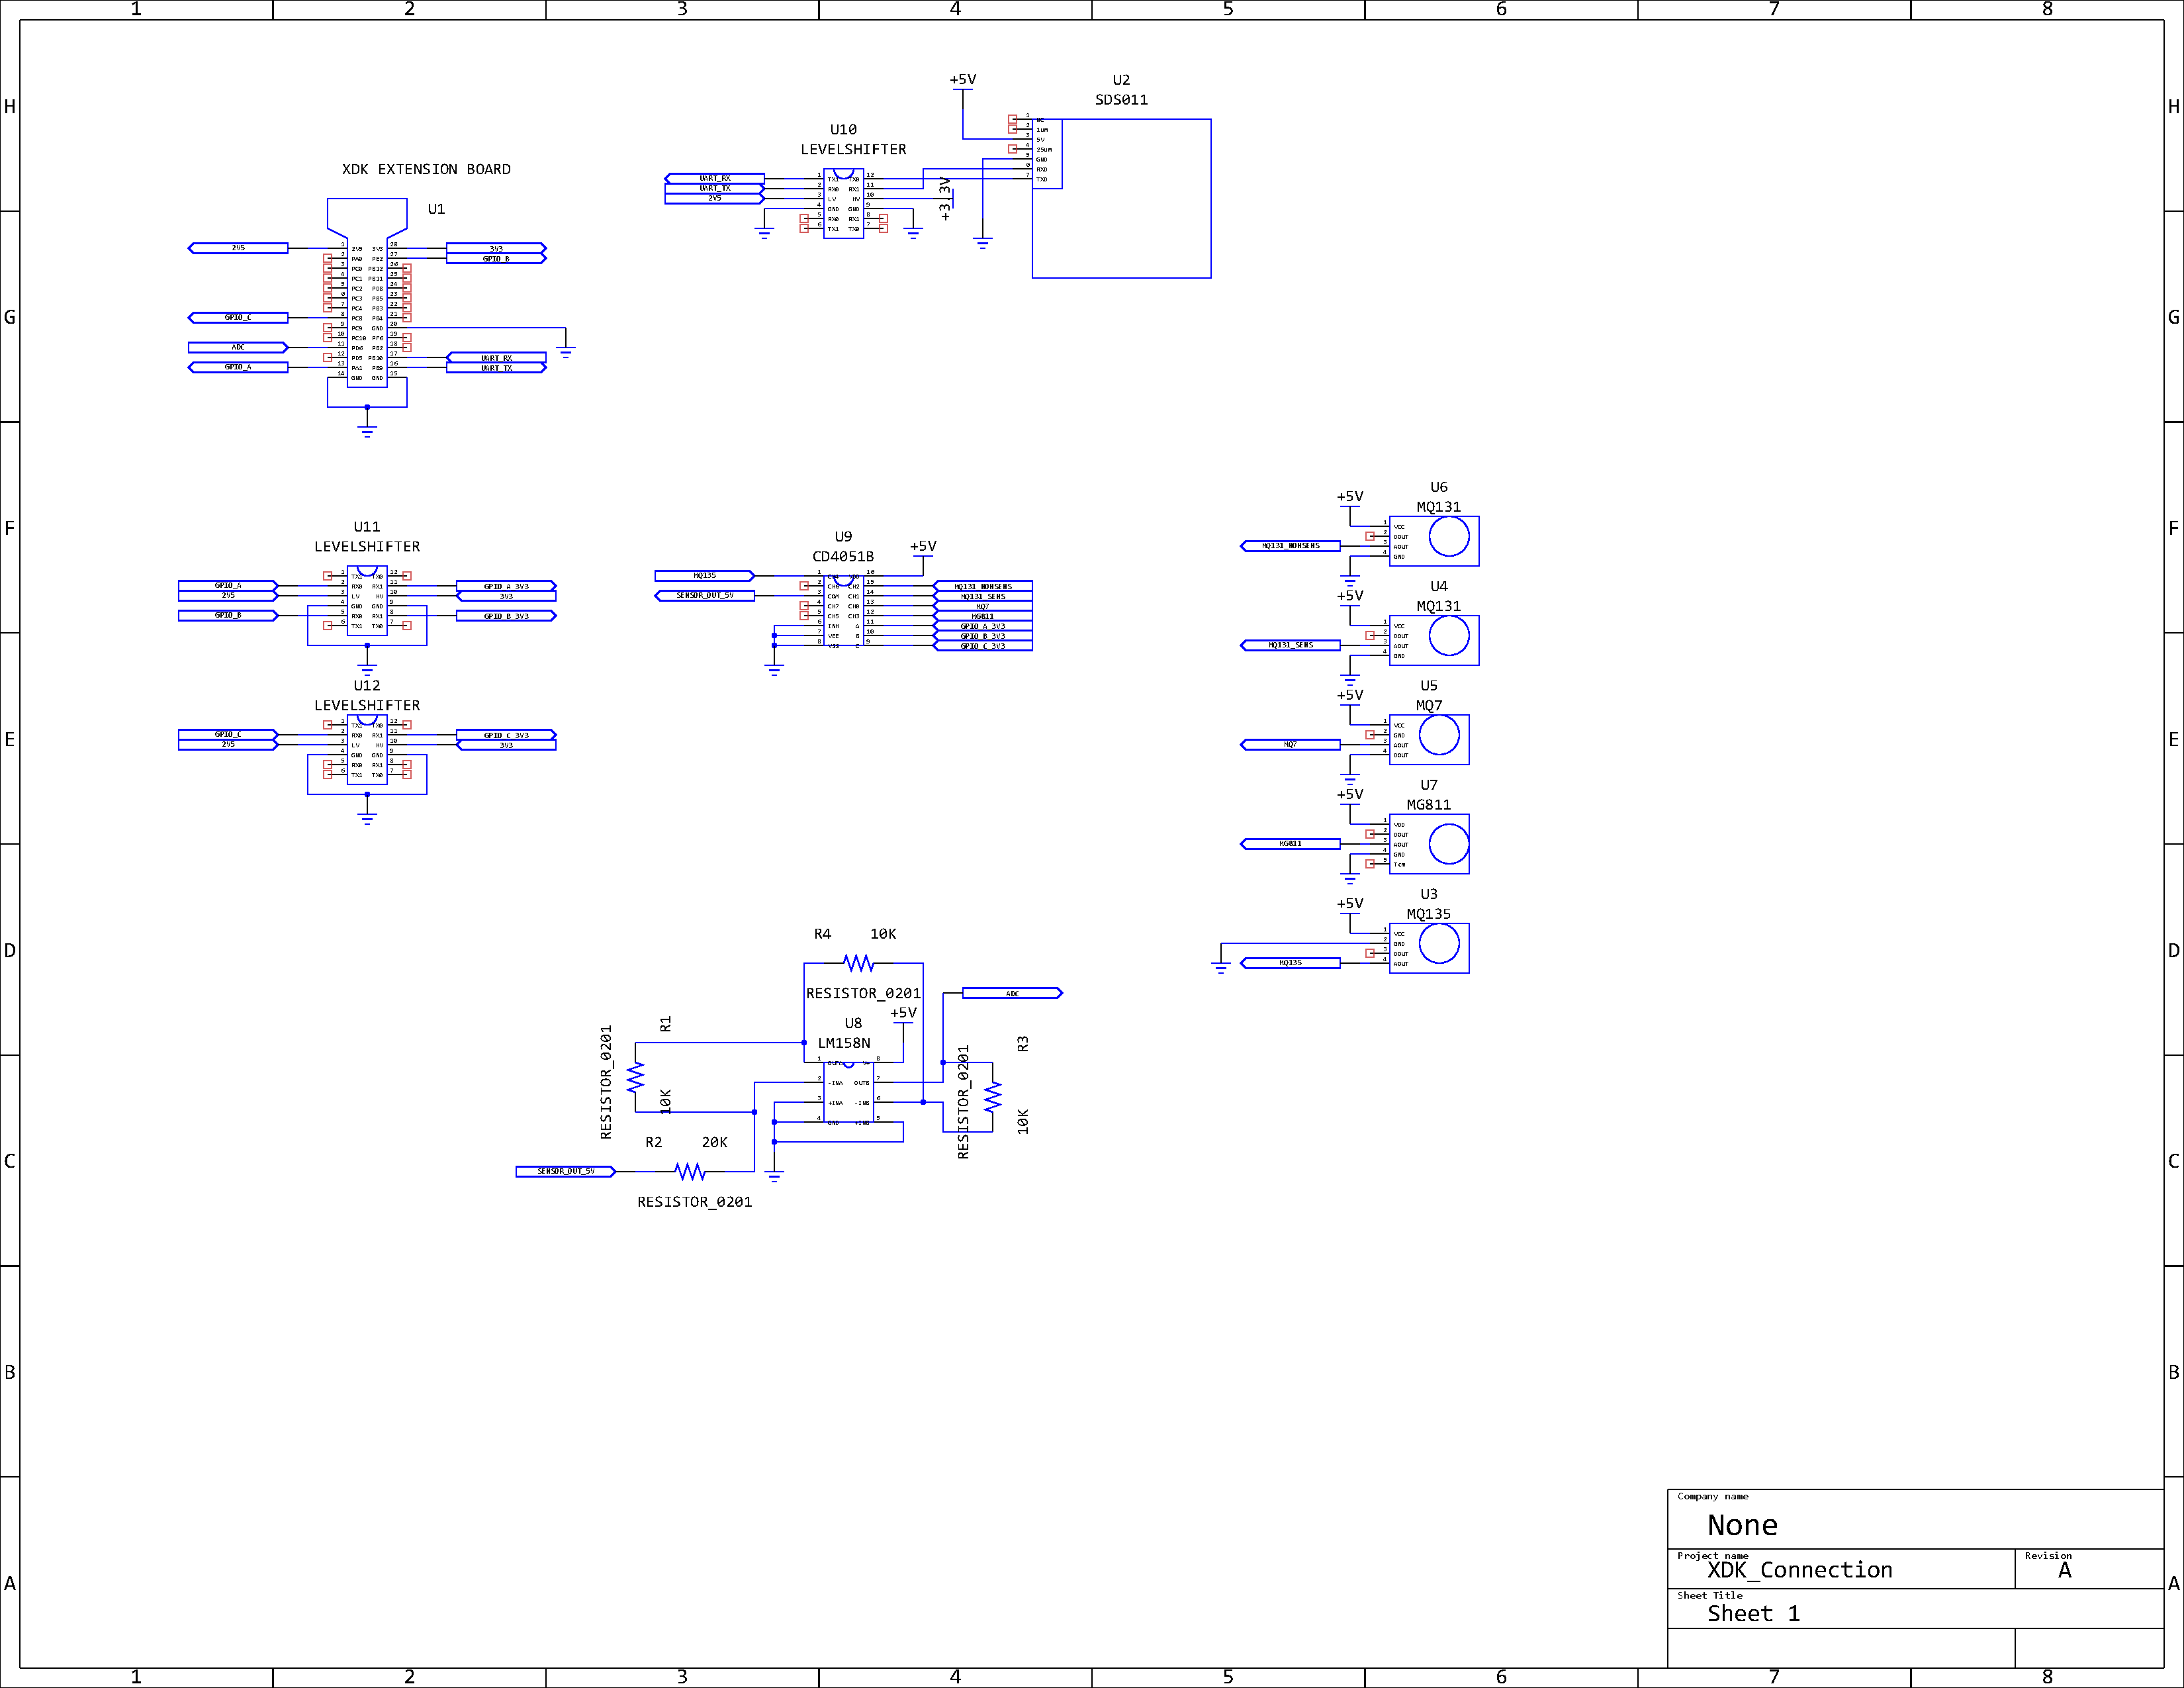
\includepdf[width=\textwidth]{Anhang/XDK_Connection_Schematic.pdf}
\pagebreak


	
\end{document}
